\documentclass[11pt,a4paper]{article}

% --- Paquetes Esenciales ---
\usepackage[utf8]{inputenc}
\usepackage[T1]{fontenc}
\usepackage{lmodern}
\usepackage[spanish,es-tabla]{babel}
\usepackage[margin=2.5cm]{geometry}
\usepackage{amsmath,amsfonts,amssymb}
\usepackage{graphicx}
\usepackage{booktabs}
\usepackage[expansion=false]{microtype}
\usepackage{float}
\usepackage{caption}
\usepackage{subcaption}
\usepackage{xcolor}
\usepackage{url}
\usepackage{hyperref}
\usepackage{natbib}
\usepackage{enumitem}
\usepackage{tabularx}
\usepackage{array}

% Permitir saltos de línea en URLs en guiones, barras, números y caracteres especiales
\def\UrlBreaks{\do\/\do\-\do\_\do\.\do\a\do\b\do\c\do\d\do\e\do\f\do\g\do\h\do\i\do\j\do\k\do\l\do\m\do\n\do\o\do\p\do\q\do\r\do\s\do\t\do\u\do\v\do\w\do\x\do\y\do\z\do\A\do\B\do\C\do\D\do\E\do\F\do\G\do\H\do\I\do\J\do\K\do\L\do\M\do\N\do\O\do\P\do\Q\do\R\do\S\do\T\do\U\do\V\do\W\do\X\do\Y\do\Z\do\0\do\1\do\2\do\3\do\4\do\5\do\6\do\7\do\8\do\9}

% --- Configuración de Enlaces y Colores ---
\definecolor{darkblue}{RGB}{11,61,145}
\definecolor{crimson}{RGB}{180,20,50}
\definecolor{forestgreen}{RGB}{20,120,40}
\hypersetup{
    colorlinks=true,
    linkcolor=darkblue,
    citecolor=darkblue,
    urlcolor=crimson,
    filecolor=forestgreen
}

% Espaciado de párrafos
\setlength{\parskip}{0.5em}
\setlength{\parindent}{0pt}

\begin{document}

% ==============================================================================
% PORTADA INSTITUCIONAL
% ==============================================================================
\begin{titlepage}
	\centering
	{\Large\bfseries UNIVERSIDAD MAYOR DE SAN ANDRÉS}\\[0.3cm]
	{\large FACULTAD DE CIENCIAS PURAS Y NATURALES}\\[0.2cm]
	{\large CARRERA DE INFORMÁTICA}\\[0.6cm]
	
	\IfFileExists{figuras/LOGOumsa.png}{
\includegraphics[width=0.38\linewidth]{figuras/LOGOumsa.png}}{%
		\IfFileExists{figuras/LOGOumsa.jpg}{\includegraphics[width=0.38\linewidth]{figuras/LOGOumsa.jpg}}{%
			\fbox{\parbox[c][3.5cm][c]{0.4\linewidth}{\centering \textbf{Logo UMSA}\\[0.2cm](figuras/LOGOumsa)}}}}\\[0.6cm]
	
	{\LARGE\bfseries Auditoría Forense Presupuestaria de los\\[0.2cm]Gobiernos Autónomos Municipales de Bolivia (2025)\\[0.35cm]
		\large Detección Multivariante de Anomalías Fiscales mediante KDD con DuckDB, Mezclas Gaussianas (GMM), Factor de Atipicidad Local (LOF) y Ley de Benford}\\[0.7cm]
	
	\begin{flushleft}
		\hspace{1.5cm}\textbf{MATERIA:} Minería de Datos (INF-398 / INF-399)\\[0.2cm]
		\hspace{1.5cm}\textbf{DOCENTE:} M.Sc. Menfy Morales Rios\\[0.2cm]
		\hspace{1.5cm}\textbf{ESTUDIANTE:}\\[0.15cm]
		\hspace{2.2cm}Cordova Avendaño Yoshua Aaron\\[0.3cm]
		\hspace{1.5cm}\textbf{INFORMACIÓN DEL PROYECTO Y ACCESO PÚBLICO:}\\[0.15cm]
		\hspace{2.2cm}\textbf{Repositorio GitHub:} \url{https://github.com/YoshGreen/GMM-LOF-DETECCION-ANOMALIAS-auditoria-fiscal-bolivia-2025}\\[0.15cm]
		\hspace{2.2cm}\textbf{Plataforma Web en Línea (Render):} \url{https://gmm-lof-deteccion-anomalias-auditoria.onrender.com/}\\[0.15cm]
		\hspace{2.2cm}\textbf{Portal Oficial de Datos (MEFP):} \url{https://abierto.economiayfinanzas.gob.bo/}\\[0.15cm]
	\end{flushleft}
	
	\vfill
	{\large\bfseries LA PAZ -- BOLIVIA}\\[0.15cm]
	{\large\bfseries Gestión Académica 2026}
\end{titlepage}

\clearpage

% ==============================================================================
% SECCIÓN PRELIMINAR: ÍNDICES FORMALES
% ==============================================================================
\pagenumbering{roman}
\setcounter{page}{1}

\tableofcontents
\clearpage

\listoffigures
\clearpage

\listoftables
\clearpage

% ==============================================================================
% CUERPO PRINCIPAL DEL INFORME
% ==============================================================================
\pagenumbering{arabic}
\setcounter{page}{1}

% ------------------------------------------------------------------------------
\section{Introducción y Contexto Institucional}
% ------------------------------------------------------------------------------
En el Estado Plurinacional de Bolivia, el proceso de descentralización y configuración del régimen autonómico, amparado en la Constitución Política del Estado de 2009 y en la Ley Marco de Autonomías y Descentralización ``Andrés Ibáñez'' (Ley N° 031), otorga a los Gobiernos Autónomos Municipales (GAM) facultades directas para formular, aprobar, ejecutar y fiscalizar sus presupuestos institucionales anuales \citep{ley031autonomias}. La estructura financiera de los 335 municipios del país está compuesta principalmente por dos vertientes: los recursos propios generados por la recaudación tributaria local (impuestos sobre bienes inmuebles, vehículos y patentes municipales) y las transferencias de recursos públicos del nivel central del Estado, destacando la Coparticipación Tributaria y el Impuesto Directo a los Hidrocarburos (IDH), catalogadas formalmente bajo la Fuente de Financiamiento 41 (Transferencias T.G.N.) \citep{mefp2025clasificador}.

A pesar del marco regulatorio establecido por la Ley de Administración y Control Gubernamentales (Ley N° 1178 - SAFCO) y las Normas Básicas del Sistema de Administración de Bienes y Servicios (D.S. N° 0181), la fiscalización pública en Bolivia ha dependido históricamente de auditorías documentales tradicionales de carácter muestral y posterior (\textit{ex-post}) ejecutadas por la Contraloría General del Estado y las unidades de auditoría interna de cada entidad. En la gestión fiscal 2025, la administración pública municipal generó más de 444.000 registros transaccionales en microdatos contables, volumen de información que satura las capacidades analíticas de las herramientas de oficina convencionales (como hojas de cálculo) y deja fuera del radar analítico patrones complejos de fraude, distorsiones operativas y desvíos presupuestarios sutiles.

El presente proyecto aplica técnicas avanzadas de Minería de Datos, Descubrimiento de Conocimiento en Bases de Datos (KDD) y Auditoría Forense Computacional sobre los registros microcontables oficiales del Ministerio de Economía y Finanzas Públicas \citep{mefp_datosabiertos}, implementando modelos de aprendizaje no supervisado basados en densidades probabilísticas (GMM) y distancias geométricas locales (LOF) para identificar irregularidades presupuestarias de forma objetiva, científica y reproducible. Todo el pipeline de procesamiento, scripts de cómputo, modelos y visualizaciones se encuentran publicados bajo licencia de acceso abierto en el repositorio GitHub institucional \citep{github_proyecto}, y la plataforma interactiva pericial está disponible en producción en la nube \citep{render_dashboard}.

\begin{table}[H]
\centering
\small
\begin{tabularx}{\textwidth}{p{4.2cm}>{\raggedright\arraybackslash}X}
\hline
\textbf{Recurso del Proyecto} & \textbf{Acceso Directo e Hiperv\'inculo Oficial} \\
\hline
\textbf{Repositorio de C\'odigo:} & \url{https://github.com/YoshGreen/GMM-LOF-DETECCION-ANOMALIAS-auditoria-fiscal-bolivia-2025} \\
\textbf{Plataforma Web en L\'inea:} & \url{https://gmm-lof-deteccion-anomalias-auditoria.onrender.com/} \\
\textbf{Portal de Datos MEFP:} & \url{https://abierto.economiayfinanzas.gob.bo/} \\
\textbf{Entorno de C\'omputo:} & R 4.4, DuckDB, \texttt{mclust} (GMM), \texttt{dbscan} (LOF), \texttt{bslib}, Docker \\
\hline
\end{tabularx}
\caption{Enlaces institucionales y acceso p\'ublico a los artefactos de la investigaci\'on.}
\label{tab:enlaces_proyecto}
\end{table}

% ------------------------------------------------------------------------------
\section{Planteamiento del Problema y Justificación}
% ------------------------------------------------------------------------------

\subsection{Planteamiento del Problema}
La auditoría y supervisión del gasto público municipal en Bolivia enfrenta tres problemas metodológicos críticos:
\begin{enumerate}[label=\textbf{\alph*)}]
    \item \textbf{El sesgo de escala en la fiscalización tradicional:} Cuando los órganos de control fiscal evalúan anomalías o seleccionan entidades para auditorías especiales, suelen basarse en umbrales monetarios absolutos o en técnicas estadísticas univariadas simples (como el criterio de Tukey sobre montos brutos). Este enfoque genera un severo sesgo de escala: clasifica automáticamente como ``atípicos'' a los municipios metropolitanos del eje central (Santa Cruz de la Sierra, La Paz, El Alto, Cochabamba) debido al volumen demográfico y magnitud de sus presupuestos, mientras que municipios medianos y rurales con graves irregularidades contables (parálisis de obras, desvío de partidas o deudas flotantes desproporcionadas) quedan encubiertos por su reducido presupuesto nominal.
    \item \textbf{Invisibilidad de anomalías multivariantes complejas:} Las irregularidades fiscales casi nunca se manifiestan como una sola cifra aislada fuera de rango; corresponden más bien a combinaciones simultáneas y patológicas de múltiples variables. Por ejemplo, una entidad puede presentar una ejecución presupuestaria aparentemente normal (80\%), pero sostener al mismo tiempo un 0\% de inversión en obras de infraestructura real, una deuda flotante extrema de compromisos no pagados y una violación de las leyes estadísticas de distribución numérica en sus comprobantes de egreso.
    \item \textbf{Limitación computacional ante datos masivos:} Los repositorios de datos abiertos del MEFP registran cientos de miles de transacciones contables detalladas. Procesar estos volúmenes con herramientas estadísticas tradicionales en memoria RAM suele provocar cuellos de botella y pérdidas de rendimiento, obligando a los analistas a realizar muestreos selectivos subjetivos que diluyen el poder probatorio de la auditoría.
\end{enumerate}

\subsection{Justificación}
\begin{itemize}[noitemsep]
    \item \textbf{Justificación Técnica y Computacional:} La incorporación de motores analíticos columnares modernos (\texttt{DuckDB}) permite procesar la totalidad del universo transaccional en disco mediante streaming sin desbordar la memoria principal, garantizando una ingesta reproducible y exhaustiva de los microdatos.
    \item \textbf{Justificación Metodológica en Minería de Datos:} La combinación sinérgica de modelos paramétricos de densidad global (Mezclas Gaussianas - GMM) con modelos no paramétricos de densidad local (Factor de Atipicidad Local - LOF) permite capturar anomalías en diferentes escalas topológicas del espacio fiscal, superando las restricciones de los métodos basados únicamente en distancias euclidianas globales.
    \item \textbf{Justificación Social e Institucional:} El presupuesto municipal representa la vía fundamental para satisfacer necesidades de salud, educación, saneamiento e infraestructura en las comunidades de Bolivia. La detección temprana y automatizada de señales de alerta de corrupción, fraccionamiento de contratos y parálisis de inversión proporciona herramientas de decisión directas para la Contraloría General del Estado, el Viceministerio de Presupuesto y la sociedad civil.
\end{itemize}

% ------------------------------------------------------------------------------
\section{Objetivos del Proyecto}
% ------------------------------------------------------------------------------

\subsection{Objetivo General}
Desarrollar e implementar un marco computacional integral de minería de datos y auditoría forense para la detección multivariante de anomalías presupuestarias y patrones atípicos de gasto e ingreso en los 335 Gobiernos Autónomos Municipales de Bolivia durante la gestión fiscal 2025, mediante la integración de procesamiento en disco con DuckDB, Modelos de Mezclas Gaussianas (GMM), Factor de Valor Atípico Local (LOF), pruebas forenses de Benford y una plataforma interactiva en R Shiny.

\subsection{Objetivos Específicos}
\begin{enumerate}[label=\textbf{\arabic*.}]
    \item \textbf{Ingesta y Poda Estructural:} Implementar un pipeline eficiente de extracción, transformación y limpieza con DuckDB sobre los microdatos contables crudos de gastos e ingresos del MEFP (más de 444.000 filas), generando un registro de auditoría de integridad contable y cruce determinístico sobre los 335 GAMs.
    \item \textbf{Ingeniería de Ratios Invariantes:} Formular y computar una matriz de 9 indicadores financieros relativos normalizados que eliminen el sesgo poblacional y dimensional, permitiendo comparaciones objetivas entre municipios rurales y capitales departamentales.
    \item \textbf{Evaluación de Línea Base Univariada:} Demostrar formal y empíricamente las limitaciones del análisis univariado clásico (criterio de Tukey $IQR$ y puntuaciones $Z$) sobre montos brutos frente al análisis de ratios normalizados.
    \item \textbf{Segmentación y Modelado Probabilístico (GMM):} Ajustar modelos de mezclas gaussianas mediante el algoritmo EM, seleccionando la estructura de covarianza y número óptimo de componentes regímenes ($G$) con el criterio de información bayesiano (BIC), e identificar anomalías globales de baja log-densidad.
    \item \textbf{Modelado de Densidad Local (LOF):} Aplicar el algoritmo Local Outlier Factor evaluando la estabilidad y sensibilidad multiescala de los scores frente a variaciones en el parámetro de vecindad ($minPts \in \{10, 15, 20, 30\}$).
    \item \textbf{Matriz de Consenso y Proyección PCA:} Construir un espacio latente mediante Análisis de Componentes Principales (PCA) y triangular las alertas de GMM y LOF para aislar un grupo prioritario de municipios en consenso de alto riesgo.
    \item \textbf{Auditoría Forense de Microdatos:} Ejecutar sobre los municipios en consenso la prueba de conformidad con la Ley de Benford (primer dígito, Chi-cuadrado y MAD de Nigrini), el test de transacciones duplicadas idénticas (alertas de fraccionamiento bajo el D.S. 0181) y la descomposición del gasto por objeto contable.
    \item \textbf{Plataforma Interactiva de Monitoreo:} Diseñar y desplegar una aplicación web interactiva en R Shiny (\texttt{dashboard/app.R}) con sistema visual \textit{Dark Telemetry}, componentes dinámicos de filtrado, proyecciones interactivas 2D/3D y expedientes municipales descargables para auditores públicos.
\end{enumerate}

% ------------------------------------------------------------------------------
\section{Marco Teórico y Fundamentos Metodológicos}
% ------------------------------------------------------------------------------

\subsection{Taxonomía de Valores Atípicos en Finanzas Públicas}
De acuerdo con la formalización de \citet{chandola2009anomaly}, un valor atípico o anomalía es un patrón en los datos que no se ajusta a la noción general de comportamiento normal. En auditoría fiscal se distinguen:
\begin{itemize}[noitemsep]
    \item \textbf{Anomalías Globales:} Observaciones que se encuentran sustancialmente apartadas de la totalidad de la masa de datos. Representan municipios con comportamientos presupuestarios atípicos respecto al estándar nacional.
    \item \textbf{Anomalías Contextuales:} Puntos que resultan anómalos únicamente en un contexto específico determinado por variables de control (por ejemplo, un municipio rural que gasta en servicios no personales como una capital metropolitana).
    \item \textbf{Anomalías Locales:} Municipios cuya densidad en el espacio multivariante es marcadamente menor que la de su vecindario más próximo, aun cuando sus indicadores no alcancen los extremos de la distribución global.
\end{itemize}

\subsection{Línea Base Univariada: Regla de Tukey y Puntuación Z}
Como punto de comparación clásico \citep{tukey1977eda}, se establece la detección univariada basada en cuartiles:
\begin{align}
    \text{Límite Atípico Leve:} & \quad [Q_1 - 1,5 \times IQR, \; Q_3 + 1,5 \times IQR] \\
    \text{Límite Atípico Extremo:} & \quad [Q_1 - 3,0 \times IQR, \; Q_3 + 3,0 \times IQR]
\end{align}
donde $IQR = Q_3 - Q_1$. Complementariamente, la puntuación normalizada $Z = (x - \bar{x})/s$ identifica observaciones con $|Z| > 2$ (desviación moderada) o $|Z| > 3$ (desviación extrema).

\subsection{Modelos de Mezclas Gaussianas (GMM) y Algoritmo EM}
Los Modelos de Mezclas Gaussianas asumen que una distribución multivariante $p(\mathbf{x})$ se genera mediante la combinación lineal convexa de $G$ densidades normales \citep{scrucca2016mclust}:
\begin{equation}
    p(\mathbf{x} \mid \boldsymbol{\theta}) = \sum_{k=1}^{G} \pi_k \, \mathcal{N}(\mathbf{x} \mid \boldsymbol{\mu}_k, \boldsymbol{\Sigma}_k)
\end{equation}
donde $\pi_k$ representa el peso del componente $k$ ($\sum \pi_k = 1, \pi_k \ge 0$), $\boldsymbol{\mu}_k$ es el centroide o vector de medias y $\boldsymbol{\Sigma}_k$ es la matriz de covarianza.

La estimación de los parámetros se realiza iterativamente mediante el algoritmo de Esperanza-Maximización (EM) \citep{dempster1977em}. En el paso E se estiman las probabilidades posteriores de pertenencia $\tau_{ik}$:
\begin{equation}
    \tau_{ik} = \frac{\pi_k \, \mathcal{N}(\mathbf{x}_i \mid \boldsymbol{\mu}_k, \boldsymbol{\Sigma}_k)}{\sum_{j=1}^G \pi_j \, \mathcal{N}(\mathbf{x}_i \mid \boldsymbol{\mu}_j, \boldsymbol{\Sigma}_j)}
\end{equation}
En el paso M se actualizan los estimadores ponderados de $\pi_k, \boldsymbol{\mu}_k$ y $\boldsymbol{\Sigma}_k$. La selección del modelo óptimo (familia geométrica de covarianza y número de grupos $G$) se determina maximizando el Criterio de Información Bayesiano (BIC) \citep{raftery1995bic}:
\begin{equation}
    \text{BIC} = 2 \ln \hat{L} - \nu \ln(n)
\end{equation}
donde $\hat{L}$ es la verosimilitud maximizada, $\nu$ es el número de parámetros independientes estimados y $n$ el número de observaciones. Las anomalías globales y contextuales se detectan evaluando la log-densidad conjunta $\ln p(\mathbf{x}_i)$, identificando como sospechosos a los municipios en el percentil inferior ($< 5\%$).

\subsection{Factor de Valor Atípico Local (LOF)}
Propuesto por \citet{breunig2000lof}, el algoritmo LOF no asume una distribución paramétrica subyacente y calcula la densidad local de un punto respecto a sus $k$ vecinos más cercanos ($N_k(\mathbf{p})$). La distancia de alcanzabilidad entre $\mathbf{p}$ y $\mathbf{o}$ se define como:
\begin{equation}
    \text{reach-dist}_k(\mathbf{p}, \mathbf{o}) = \max \{ k\text{-distancia}(\mathbf{o}), d(\mathbf{p}, \mathbf{o}) \}
\end{equation}
La densidad de alcanzabilidad local ($lrd_k$) se obtiene como el recíproco del promedio de distancias de alcanzabilidad:
\begin{equation}
    lrd_k(\mathbf{p}) = \left[ \frac{\sum_{\mathbf{o} \in N_k(\mathbf{p})} \text{reach-dist}_k(\mathbf{p}, \mathbf{o})}{|N_k(\mathbf{p})|} \right]^{-1}
\end{equation}
El score LOF es el cociente promedio de las densidades de los vecinos sobre la densidad del punto:
\begin{equation}
    \text{LOF}_k(\mathbf{p}) = \frac{\sum_{\mathbf{o} \in N_k(\mathbf{p})} \frac{lrd_k(\mathbf{o})}{lrd_k(\mathbf{p})}}{|N_k(\mathbf{p})|}
\end{equation}
Un score cercano a 1 indica pertenencia a un conglomerado uniforme; valores de $\text{LOF} > 1,5$ señalan aislamiento local estadísticamente relevante.

\subsection{Ley de Benford y Criterios Forenses de Nigrini}
La Ley de Benford \citep{benford1938law} establece que en colecciones de números formadas de manera natural y sin topes artificiales, la probabilidad teórica de que el primer dígito significativo sea $d \in \{1, \dots, 9\}$ sigue la ley logarítmica:
\begin{equation}
    P(d) = \log_{10}\left(1 + \frac{1}{d}\right)
\end{equation}
Para contrastar la hipótesis de conformidad forense se calculan el estadístico Chi-cuadrado ($\chi^2 = n \sum_{d=1}^9 \frac{(f_d^{\text{obs}} - P(d))^2}{P(d)}$ con 8 g.l.) y la Desviación Absoluta Media (MAD) \citep{nigrini2012benford}:
\begin{equation}
    \text{MAD} = \frac{1}{9} \sum_{d=1}^9 \left| f_d^{\text{obs}} - P(d) \right|
\end{equation}
Bajo los estándares de auditoría forense de \citet{nigrini2012benford}:
\begin{itemize}[noitemsep]
    \item $\text{MAD} \le 0,006$: Conformidad cercana (\textit{Close conformity}).
    \item $0,006 < \text{MAD} \le 0,012$: Conformidad aceptable (\textit{Acceptable conformity}).
    \item $0,012 < \text{MAD} \le 0,015$: Conformidad marginal (\textit{Marginally acceptable conformity}).
    \item $\text{MAD} > 0,015$: No conformidad o violación (\textit{Nonconformity}), indicador de distorsión antrópica o manipulación documental.
\end{itemize}

\subsection{Marco Legal: Ley 1178 (SAFCO) y D.S. 0181 (NB-SABS)}
En el ordenamiento jurídico boliviano, el Sistema de Contratación de Bienes y Servicios (D.S. N° 0181) prohíbe taxativamente el fraccionamiento deliberado del gasto orientado a eludir licitaciones públicas transparentes \citep{ds0181}. Los techos para Contratación Menor se fijan en compras de hasta Bs. 50.000 (con subtramos operativos habituales en Bs. 20.000). La reiteración atípica de comprobantes exactamente por debajo o en estos límites constituye una señal de alerta forense vinculada a la responsabilidad civil y penal prevista en la Ley N° 1178 (SAFCO) \citep{ley1178safco}.

% ------------------------------------------------------------------------------
\section{Desarrollo Metodológico y Pipeline KDD}
% ------------------------------------------------------------------------------

\subsection{Flujo de Trabajo KDD}
El proceso de Descubrimiento de Conocimiento en Bases de Datos (KDD) \citep{fayyad1996kdd} se organizó en cinco fases secuenciales e iterativas:
\begin{enumerate}[label=\textbf{\arabic*.}]
    \item \textbf{Selección de Datos:} Ingesta de los microdatos abiertos oficiales descargados del portal del Ministerio de Economía y Finanzas Públicas \citep{mefp_datosabiertos} (\url{https://abierto.economiayfinanzas.gob.bo/}): \texttt{presupuesto\_gasto\_gestion\_2025.csv} (408,3 MB, 429.753 partidas) y \texttt{presupuesto\_ingreso\_gestion\_2025.csv} (8,8 MB, 14.644 rubros).
    \item \textbf{Preprocesamiento y Auditoría:} Filtrado estructural de subárea (\texttt{entidad\_sigla\_subarea == 'GAM'}), gestión 2025, tratamiento de valores nulos con \texttt{coalesce} y detección de inconsistencias lógicas.
    \item \textbf{Transformación e Ingeniería de Atributos:} Consolidación a nivel entidad y construcción de 9 ratios fiscales relativos normalizados con \texttt{scale()}.
    \item \textbf{Minería de Datos Multivariante:} Ajuste simultáneo de modelos GMM (\texttt{mclust}) y LOF (\texttt{dbscan}) con proyección en componentes principales (PCA).
    \item \textbf{Evaluación y Auditoría Forense Drill-Down:} Extracción de microdatos para los municipios priorizados en consenso y ejecución de pruebas de Benford, fraccionamiento y estructura de compras.
\end{enumerate}

\subsection{Poda Estructural y Auditoría Contable con DuckDB}
Para garantizar la viabilidad computacional sin requerir memoria RAM masiva, se utilizó el paquete \texttt{duckdb} en R. Las consultas analíticas se ejecutaron directamente sobre disco. Como resume la Tabla \ref{tab:auditoria_limpieza}, se procesaron 429.753 partidas de gastos y 14.644 rubros de ingresos, filtrando 263.893 y 9.436 registros municipales respectivamente, correspondientes con exactitud a los 335 GAMs del país.

\begin{table}[htbp]
\centering
\small
\caption{Auditor\'ia de Integridad Contable y Filtrado KDD (Gesti\'on 2025)}
\label{tab:auditoria_limpieza}
\begin{tabular}{lrr}
\hline
\textbf{M\'etrica de Auditor\'ia / Poda Fiscal} & \textbf{Presupuesto Gastos} & \textbf{Presupuesto Ingresos} \\
\hline
Filas Totales en CSV Crudo & 429.753 & 14.644 \\
Filas Gesti\'on 2025 & 429.753 & 14.644 \\
Filas Gobiernos Municipales (GAM) & 263.893 & 9.436 \\
Municipios Identificados (Entidades \'Unicas) & 335 & 335 \\
Valores Nulos en Campos Monetarios & 0 & 0 \\
Registros con Reversiones (Montos Negativos) & 3 & 2 \\
Inconsistencias Contables Detectadas & 3843 & 4585 \\
\textbf{GAMs Consolidados en Matriz Final} & \multicolumn{2}{c}{\textbf{335}} \\
\hline
\end{tabular}
\end{table}


El análisis de integridad contable inicial arrojó cero valores nulos en columnas monetarias esenciales, 1 partida de gasto devengado negativo, 498 partidas con presupuesto vigente negativo (reversiones contables), y 306 partidas donde el monto pagado excedió al devengado. En ingresos se registraron 1.366 registros con presupuesto vigente cero pero recaudación efectiva positiva, provenientes de transferencias extraordinarias no presupuestadas en el POA inicial.

\subsection{Diccionario de Datos y Selección de Características}
Los conjuntos de datos crudos publicados por el Ministerio de Economía y Finanzas Públicas (MEFP) poseen una estructura multidimensional altamente desagregada, compuesta originalmente por 67 atributos en el archivo de Gastos y 42 atributos en el de Ingresos (109 columnas en total). En concordancia con los principios del proceso KDD \citep{fayyad1996kdd}, someter el modelo de minería a la totalidad de campos provocaría una degradación severa por la ``maldición de la dimensionalidad'', redundancia semántica y sobreajuste.

Por tanto, se aplicó una estrategia de selección de características basada en los siguientes criterios contables y matemáticos:
\begin{enumerate}[label=\textbf{\alph*)}]
    \item \textbf{Variables Conservadas e Involucradas:} Se seleccionaron los atributos temporales (\texttt{gestion}), los discriminadores institucionales (\texttt{entidad\_sigla\_subarea}, \texttt{entidad}), los campos geográficos (\texttt{desc\_departamento}, \texttt{desc\_municipio}), la totalidad de flujos monetarios (\texttt{inicial}, \texttt{vigente}, \texttt{devengado}, \texttt{pagado}, \texttt{percibido}), el discriminador de proyectos de inversión (\texttt{actividad = 0}), el grupo de servicios no personales (\texttt{objeto\_grupo = 20000}), la fuente de transferencias gubernamentales (\texttt{fuente = 41}) y los clasificadores de partida para la auditoría de montos duplicados en compras menores.
    \item \textbf{Variables Excluidas y Justificación:} Se descartaron las columnas que presentaban redundancia funcional (duplicidad de código numérico y texto descriptivo, como \texttt{fuente} y \texttt{desc\_fuente}), jerarquías institucionales constantes tras el filtrado municipal (\texttt{entidad\_sector}, \texttt{entidad\_area}, etc.), niveles de desagregación interna sin relevancia macrofiscal (\texttt{da}, \texttt{desc\_da}), y clasificadores sectoriales o de cuentas nacionales (\texttt{finfun\_*}, \texttt{acteco\_*}) que no inciden en la solvencia financiera, la deuda flotante ni en la detección de patrones de fraude contable.
\end{enumerate}

La Tabla \ref{tab:diccionario_datos} detalla el inventario estructurado de atributos de ambos conjuntos de datos, su tipología formal y el dictamen técnico de inclusión o exclusión analítica.

% ==============================================================================
% TABLA: DICCIONARIO DE DATOS Y SELECCIÓN DE CARACTERÍSTICAS (MEFP 2025)
% ==============================================================================

\begin{table}[H]
\centering
\scriptsize
\begin{tabularx}{\textwidth}{p{3.2cm}p{1.6cm}p{1.4cm}>{\raggedright\arraybackslash}X}
\toprule
\textbf{Campo / Atributo MEFP} & \textbf{Tipo Dato} & \textbf{Estado} & \textbf{Propósito Analítico o Justificación de Exclusión} \\
\midrule
\multicolumn{4}{l}{\textbf{A. Macrodatos de Gastos (\texttt{presupuesto\_gasto\_gestion\_2025.csv} -- 67 columnas originales)}} \\
\midrule
\texttt{gestion} & Entero & \textbf{Usado} & Filtro temporal estricto (\texttt{gestion == 2025}). \\
\texttt{entidad\_sigla\_subarea} & Texto & \textbf{Usado} & Filtro institucional para aislar Gobiernos Municipales (\texttt{'GAM'}). \\
\texttt{entidad} & Entero & \textbf{Usado} & Identificador primario único del GAM (llave de cruce relacional). \\
\texttt{entidad\_desc\_entidad} & Texto & \textbf{Usado} & Razón social oficial del Gobierno Autónomo Municipal. \\
\texttt{desc\_departamento} & Texto & \textbf{Usado} & Segmentación territorial departamental (9 departamentos). \\
\texttt{desc\_provincia}, \texttt{desc\_municipio} & Texto & \textbf{Usado} & Contexto geográfico para etiquetado forense y drill-down. \\
\texttt{inicial} & Decimal & \textbf{Usado} & Presupuesto institucional aprobado; cálculo de modificación (TMP). \\
\texttt{vigente} & Decimal & \textbf{Usado} & Techo presupuestario modificado; denominador de ejecución (TEG). \\
\texttt{devengado} & Decimal & \textbf{Usado} & Obligación económica formal; base de los ratios de gasto y Benford. \\
\texttt{pagado} & Decimal & \textbf{Usado} & Desembolso efectivo de caja; cálculo de deuda flotante exigible. \\
\texttt{actividad} & Entero & \textbf{Usado} & Separación contable: \texttt{actividad = 0} identifica inversión pública. \\
\texttt{objeto\_grupo} & Entero & \textbf{Usado} & Clasificador: grupo \texttt{20000} identifica Servicios No Personales. \\
\texttt{objeto\_partida}, \texttt{objeto\_desc\_partida} & Entero/Txt & \textbf{Usado} & Auditoría drill-down de compras y montos idénticos repetitivos. \\
\addlinespace
\texttt{entidad\_sector}, \texttt{subsector}, \texttt{area}, \texttt{subarea} (códigos y descripciones) & Varios & \textit{No Usado} & Constantes o redundantes tras el filtro inicial de subárea \texttt{'GAM'}. \\
\texttt{da}, \texttt{desc\_da} (Dirección Administrativa) & Varios & \textit{No Usado} & Nivel de desagregación interno variable no comparable entre GAMs. \\
\texttt{programa}, \texttt{desc\_programa}, \texttt{proyecto} & Varios & \textit{No Usado} & Codificación programática heterogénea; capturada por \texttt{actividad}. \\
\texttt{entidad\_transferencia} & Entero & \textit{No Usado} & Vacío o cero en la mayoría de comprobantes operativos municipales. \\
\texttt{objeto\_subgrupo}, \texttt{subpartida} (códigos y textos) & Varios & \textit{No Usado} & Alta dimensionalidad dispersa; consolidada en grupo y partida. \\
\texttt{fuente}, \texttt{organismo} (clasificador completo de financiamiento) & Varios & \textit{No Usado} & Múltiples niveles redundantes; la estructura de financiamiento clave se captura en ingresos. \\
\texttt{finfun\_*} (Finalidad y Función - 6 campos) & Varios & \textit{No Usado} & Clasificación funcional secundaria; no afecta la ejecución financiera. \\
\texttt{acteco\_*} (Actividad Económica - 6 campos) & Varios & \textit{No Usado} & Criterio de cuentas nacionales no incidente en solvencia o fraude. \\
\midrule
\multicolumn{4}{l}{\textbf{B. Macrodatos de Ingresos (\texttt{presupuesto\_ingreso\_gestion\_2025.csv} -- 42 columnas originales)}} \\
\midrule
\texttt{gestion} & Entero & \textbf{Usado} & Filtro temporal estricto (\texttt{gestion == 2025}). \\
\texttt{entidad\_sigla\_subarea} & Texto & \textbf{Usado} & Filtro institucional para aislar Gobiernos Municipales (\texttt{'GAM'}). \\
\texttt{entidad} & Entero & \textbf{Usado} & Llave foránea de unión con la base de gastos. \\
\texttt{inicial} & Decimal & \textbf{Usado} & Estimación presupuestaria inicial de recursos propios y transferencias. \\
\texttt{vigente} & Decimal & \textbf{Usado} & Presupuesto vigente de ingresos; cálculo de eficacia recaudadora. \\
\texttt{devengado} & Decimal & \textbf{Usado} & Derecho de cobro reconocido en la gestión fiscal. \\
\texttt{percibido} & Decimal & \textbf{Usado} & Recaudación efectiva líquida; cálculo del balance de caja real. \\
\texttt{fuente} & Entero & \textbf{Usado} & Identificación de Fuente \texttt{41} (Transferencias T.G.N., IDH, Coparticipación). \\
\addlinespace
\texttt{entidad\_*} (sector, subsector, área, descripciones) & Varios & \textit{No Usado} & Redundantes con la jerarquía institucional ya vinculada en gastos. \\
\texttt{rubro\_tipo}, \texttt{clase}, \texttt{cuenta}, \texttt{sub\_cuenta} (códigos y descripciones) & Varios & \textit{No Usado} & Desagregación excesiva que atomiza la recaudación sin alterar la solvencia global. \\
\texttt{grupo\_fuente}, \texttt{desc\_grupo\_fuente}, \texttt{desc\_fuente} & Varios & \textit{No Usado} & Texto explicativo redundante con el código numérico \texttt{fuente = 41}. \\
\texttt{organismo\_*} (9 campos de organismos financiadores) & Varios & \textit{No Usado} & Mayoritariamente transferencias directas del T.G.N. sin variación local. \\
\texttt{entidad\_otorgante} & Entero & \textit{No Usado} & Escaso llenado y no uniforme entre alcaldías municipales. \\
\bottomrule
\end{tabularx}
\caption{Diccionario de datos oficial (MEFP), inventario de campos y fundamentación analítica de inclusión/exclusión.}
\label{tab:diccionario_datos}
\end{table}


\subsection{Ingeniería de Características: 9 Ratios Invariantes a la Escala}
Con el fin de eliminar el sesgo de tamaño poblacional, se definieron nueve indicadores matemáticos por municipio:
\begin{enumerate}[label=\textbf{\arabic*.}]
    \item \textbf{Tasa de Ejecución del Gasto (TEG):} $\text{TEG} = \frac{\text{Gasto Devengado}}{\text{Gasto Vigente}}$. Mide la capacidad de absorción y cumplimiento de metas del gasto.
    \item \textbf{Tasa de Modificación Presupuestaria (TMP):} $\text{TMP} = \frac{\text{Gasto Vigente} - \text{Gasto Inicial}}{\text{Gasto Inicial}}$. Cuantifica la alteración de la programación fiscal inicial.
    \item \textbf{Brecha de Pago o Deuda Flotante (DF):} $\text{DF} = \frac{\text{Gasto Devengado} - \text{Gasto Pagado}}{\text{Gasto Devengado}}$. Representa la acumulación de obligaciones contraídas con contratistas y proveedores no canceladas en efectivo.
    \item \textbf{Ratio de Inversión Pública (RIP):} $\text{RIP} = \frac{\text{Devengado en Proyectos (Actividad = 0)}}{\text{Gasto Devengado}}$. Proporción del gasto canalizado a la formación bruta de capital e infraestructura frente al gasto corriente.
    \item \textbf{Ratio de Servicios No Personales (R20):} $\text{R20} = \frac{\text{Devengado Grupo 20000}}{\text{Gasto Devengado}}$. Concentración de gasto en consultorías, mantenimiento y contratos transitorios.
    \item \textbf{Balance de Caja Real (BCR):} $\text{BCR} = \frac{\text{Ingreso Percibido} - \text{Gasto Pagado}}{\text{Ingreso Percibido}}$. Posición neta de liquidez efectiva al cierre de caja.
    \item \textbf{Eficacia de Recaudación (ER):} $\text{ER} = \frac{\text{Ingreso Percibido}}{\text{Ingreso Vigente}}$. Capacidad de cobranza frente a lo programado en ingresos.
    \item \textbf{Dependencia del TGN (DEP):} $\text{DEP} = \frac{\text{Percibido Fuente 41}}{\text{Ingreso Percibido}}$. Grado de subordinación financiera ante transferencias del nivel central.
    \item \textbf{Escala Presupuestaria Logarítmica (LOGP):} $\text{LOGP} = \ln(1 + \text{Gasto Vigente})$. Factor de control dimensional.
\end{enumerate}

Todos los ratios fueron estandarizados ($\mu=0, \sigma=1$) antes de ingresar a los algoritmos de aprendizaje de máquinas.

\subsection{Demostración Empírica del Sesgo de Escala Univariado}
La Tabla \ref{tab:linea_base_univariada} y la Figura \ref{fig:sesgo_escala} demuestran con contundencia por qué la auditoría basada en cifras monetarias brutas resulta contraproducente.

\begin{table}[htbp]
\centering
\footnotesize
\caption{L\'inea Base Univariada: Comparativa de Umbrales Tukey y Z-Score (335 GAMs)}
\label{tab:linea_base_univariada}
\begin{tabular}{lrrrrrr}
\hline
\textbf{Variable Presupuestaria} & \textbf{Media} & \textbf{IQR} & \textbf{Tukey 1.5} & \textbf{Tukey 3.0} & \textbf{$|z|>2$} & \textbf{$|z|>3$} \\
\hline
\multicolumn{7}{l}{\textit{Panel A: Montos Monetarios Brutos (Sesgo de Escala)}} \\
Presupuesto Vigente (Bs.) & 7.56e+07 & 2.90e+07 & 39 & 25 & 5 & 4 \\
Gasto Devengado (Bs.) & 6.09e+07 & 2.12e+07 & 40 & 25 & 6 & 4 \\
Ingreso Percibido (Bs.) & 5.77e+07 & 2.11e+07 & 41 & 26 & 6 & 4 \\
\hline
\multicolumn{7}{l}{\textit{Panel B: Ratios Fiscales Invariantes a la Escala}} \\
Tasa de Ejecución Gasto & 0.751 & 0.155 & 1 & 0 & 13 & 1 \\
Tasa Modificación Presupuestaria & 0.631 & 0.573 & 11 & 1 & 19 & 4 \\
Brecha de Pago (Deuda Flotante) & 0.012 & 0.011 & 40 & 30 & 20 & 11 \\
Ratio de Inversión Pública & 0.253 & 0.201 & 1 & 0 & 10 & 1 \\
Ratio Serv. No Personales (Gr. 20000) & 0.274 & 0.154 & 0 & 0 & 11 & 0 \\
Balance de Caja Real & 0.024 & 0.113 & 20 & 3 & 20 & 6 \\
Eficacia de Recaudación & 0.765 & 0.135 & 5 & 0 & 14 & 1 \\
Dependencia de Transferencias TGN & 0.825 & 0.201 & 9 & 0 & 16 & 3 \\
\hline
\end{tabular}
\end{table}


\begin{figure}[H]
    \centering
    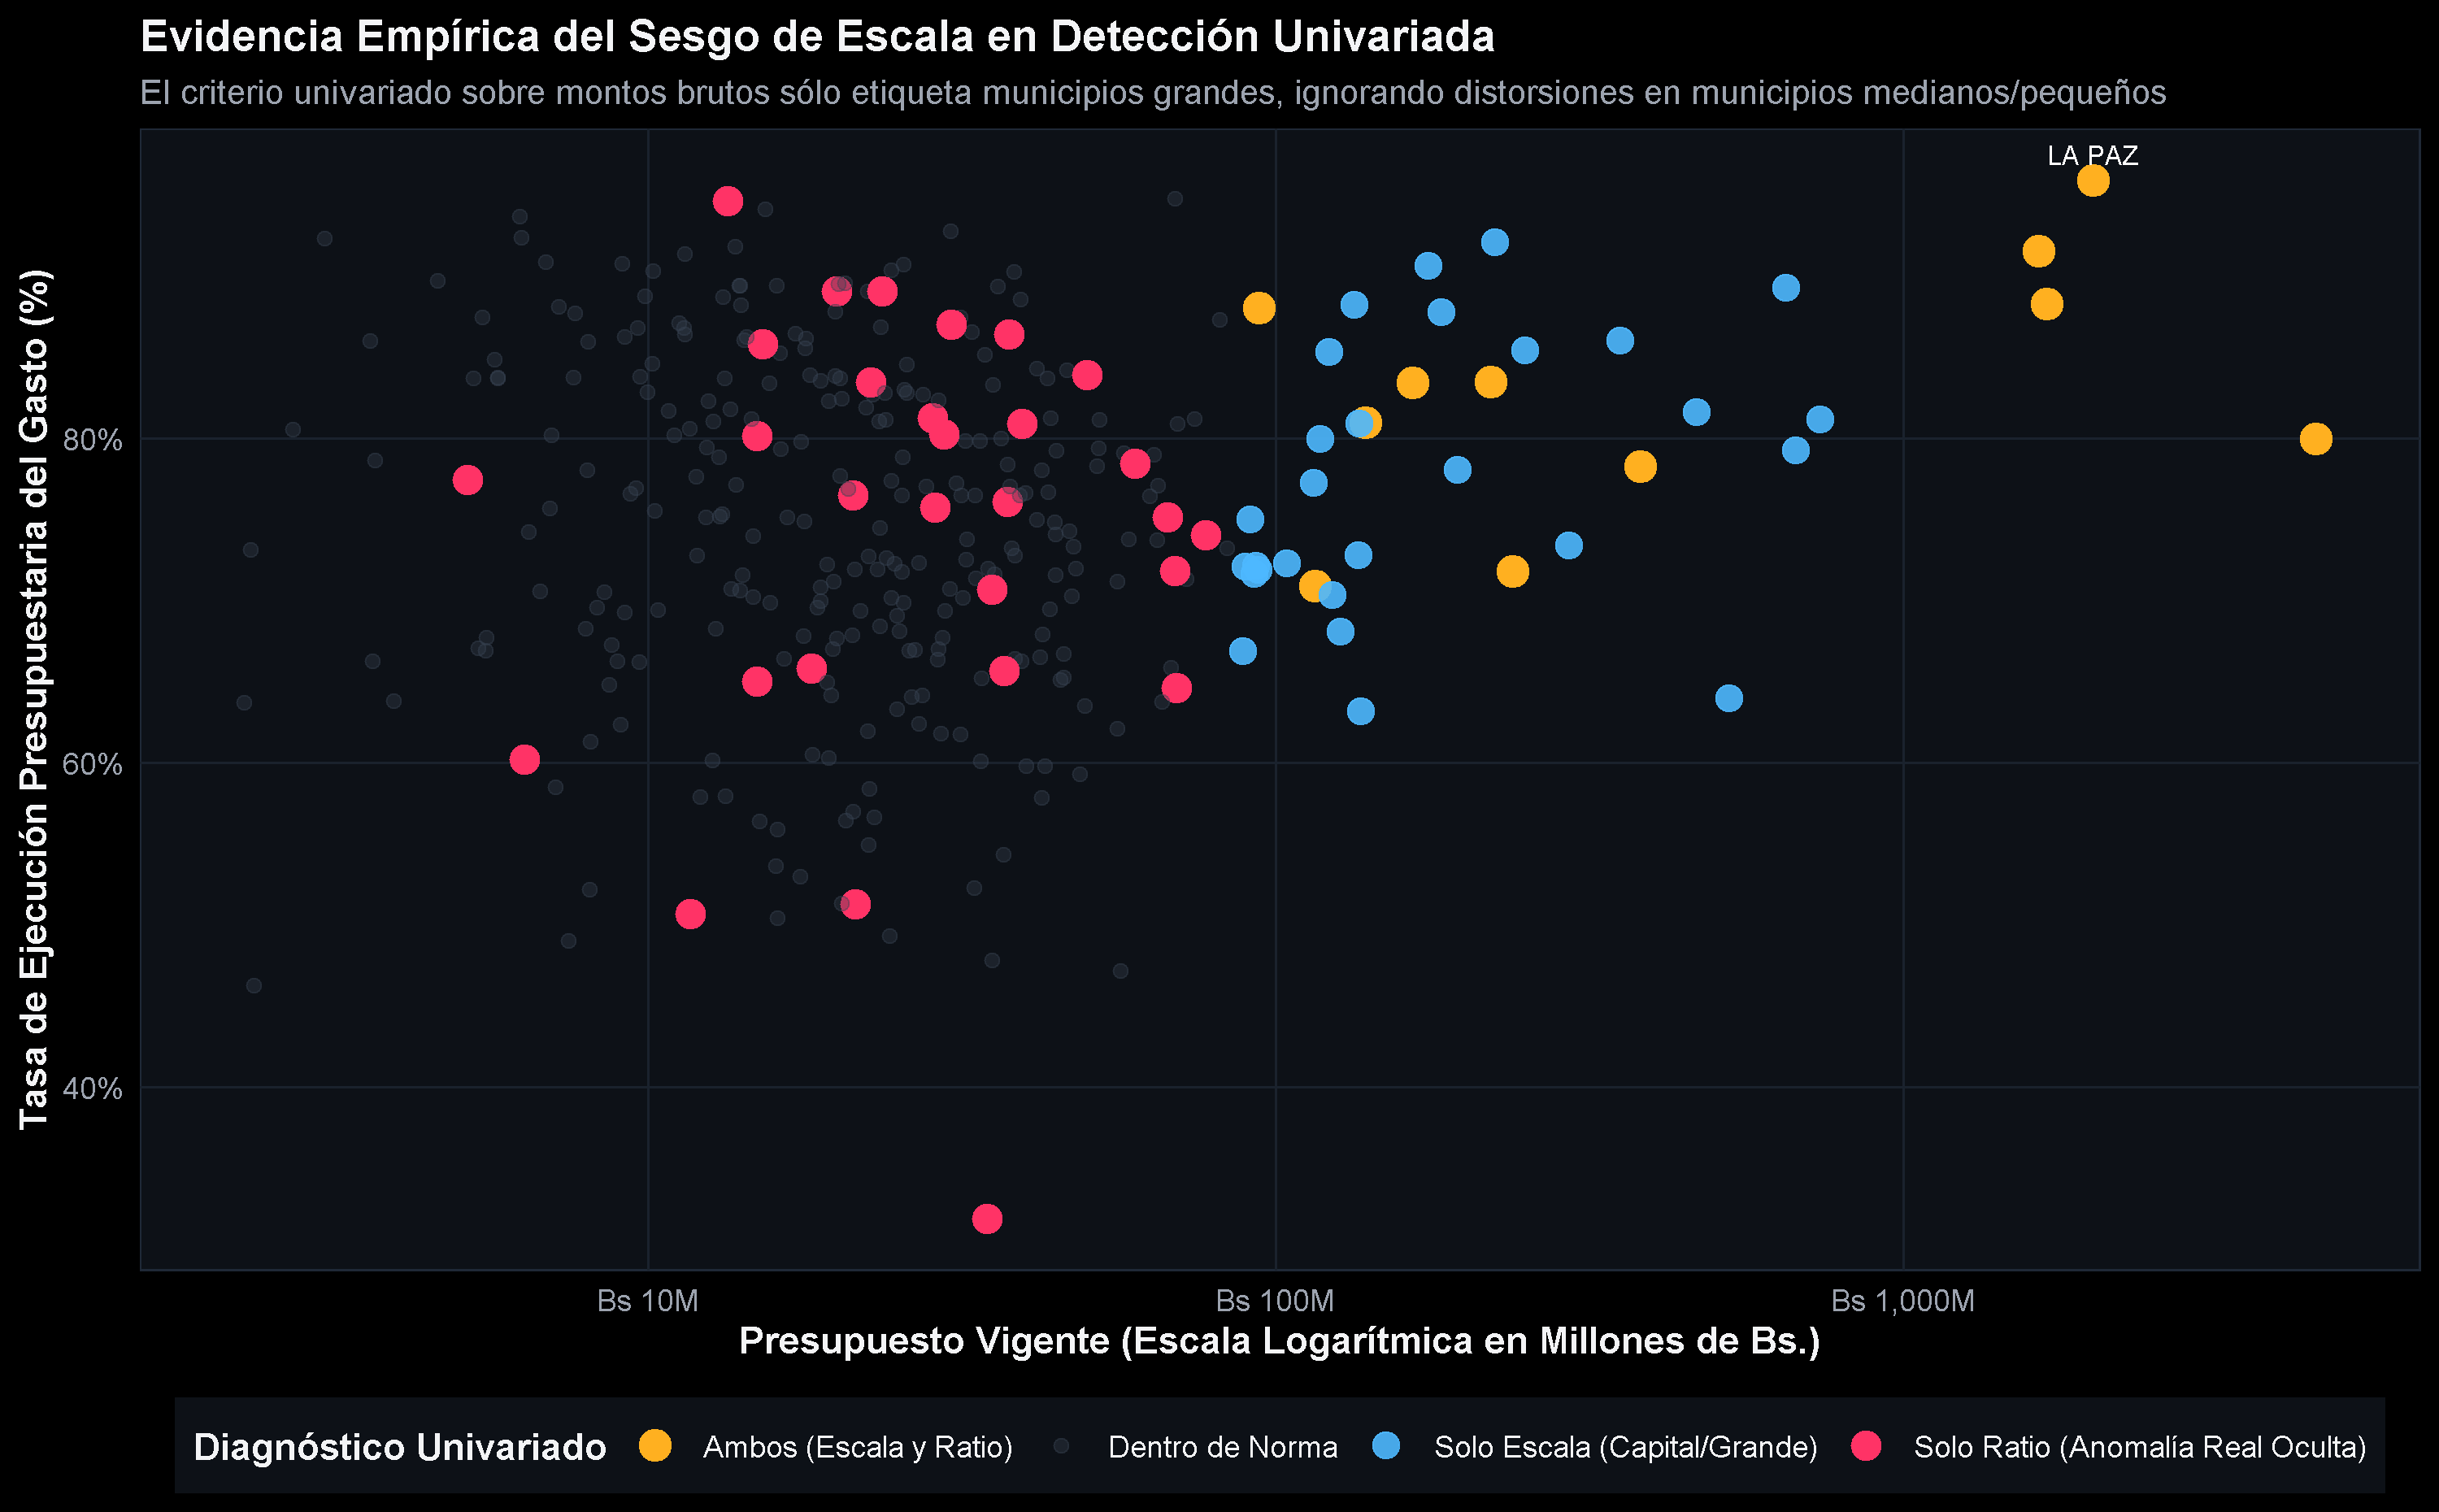
\includegraphics[width=0.92\textwidth]{figuras/fig_01_sesgo_escala_univariado.png}
    \caption{Demostración empírica del sesgo de escala: los criterios sobre montos brutos (Tukey/Z) señalan a las grandes ciudades (falsos positivos), mientras que los ratios relativos descubren distorsiones operativas críticas.}
    \label{fig:sesgo_escala}
\end{figure}

Al aplicar el criterio de Tukey sobre el presupuesto vigente bruto, se aíslan 39 municipios, todos ellos correspondientes a capitales departamentales o urbes metropolitanas (Tabla \ref{tab:top_atipicos_univariados}). Sin embargo, estas ciudades operan con ratios normales (ejecuciones entre 80\% y 90\%). En contraste, los indicadores relativos de comportamiento descubren distorsiones severas en municipios no metropolitanos: Chulumani ejecuta apenas 31,87\% de su presupuesto y acumula 16,20\% de deuda flotante; Caquiaviri sostiene 15,95\% de deuda flotante impaga; y Tahua asigna 0\% de su presupuesto a inversión pública real.

\begin{table}[htbp]
\centering
\caption{Demostraci\'on del Sesgo de Escala: Grandes Ciudades vs. Distorsiones Ocultas}
\label{tab:top_atipicos_univariados}
\resizebox{\textwidth}{!}{%
\begin{tabular}{llrrrr}
\hline
\textbf{Municipio} & \textbf{Departamento} & \textbf{Ppto. Vigente (Bs.)} & \textbf{Ejec. (\%)} & \textbf{Deuda Flot. (\%)} & \textbf{Diagn\'ostico Univ.} \\
\hline
\multicolumn{6}{l}{\textit{Se\~nalados por Tukey en Montos Brutos (Falsos Positivos de Escala)}} \\
Gobierno Aut\'onomo Municipal De Santa Cruz De La Sierra & SANTA CRUZ & 4.558.779.115 & 80.0\% & 17.77\% & Solo Gran Escala \\
Gobierno Aut\'onomo Municipal De La Paz & LA PAZ & 2.009.174.841 & 95.9\% & 7.48\% & Solo Gran Escala \\
Gobierno Aut\'onomo Municipal De El Alto De La Paz & LA PAZ & 1.699.038.807 & 88.3\% & 10.64\% & Solo Gran Escala \\
\hline
\multicolumn{6}{l}{\textit{Se\~nalados por Ratios Fiscales pero Omitidos por Escala (Verdaderas Distorsiones)}} \\
Gobierno Aut\'onomo Municipal De Santa Cruz De La Sierra & SANTA CRUZ & 4.558.779.115 & 80.0\% & 17.77\% & Alta Deuda Flotante \\
Gobierno Aut\'onomo Municipal De Chulumani (Villa De La Libertad) & LA PAZ & 34.702.480 & 31.9\% & 16.20\% & Alta Deuda Flotante \\
Gobierno Aut\'onomo Municipal De Caquiaviri & LA PAZ & 19.972.963 & 89.1\% & 15.95\% & Alta Deuda Flotante \\
\hline
\end{tabular}%
}
\end{table}


\begin{figure}[H]
    \centering
    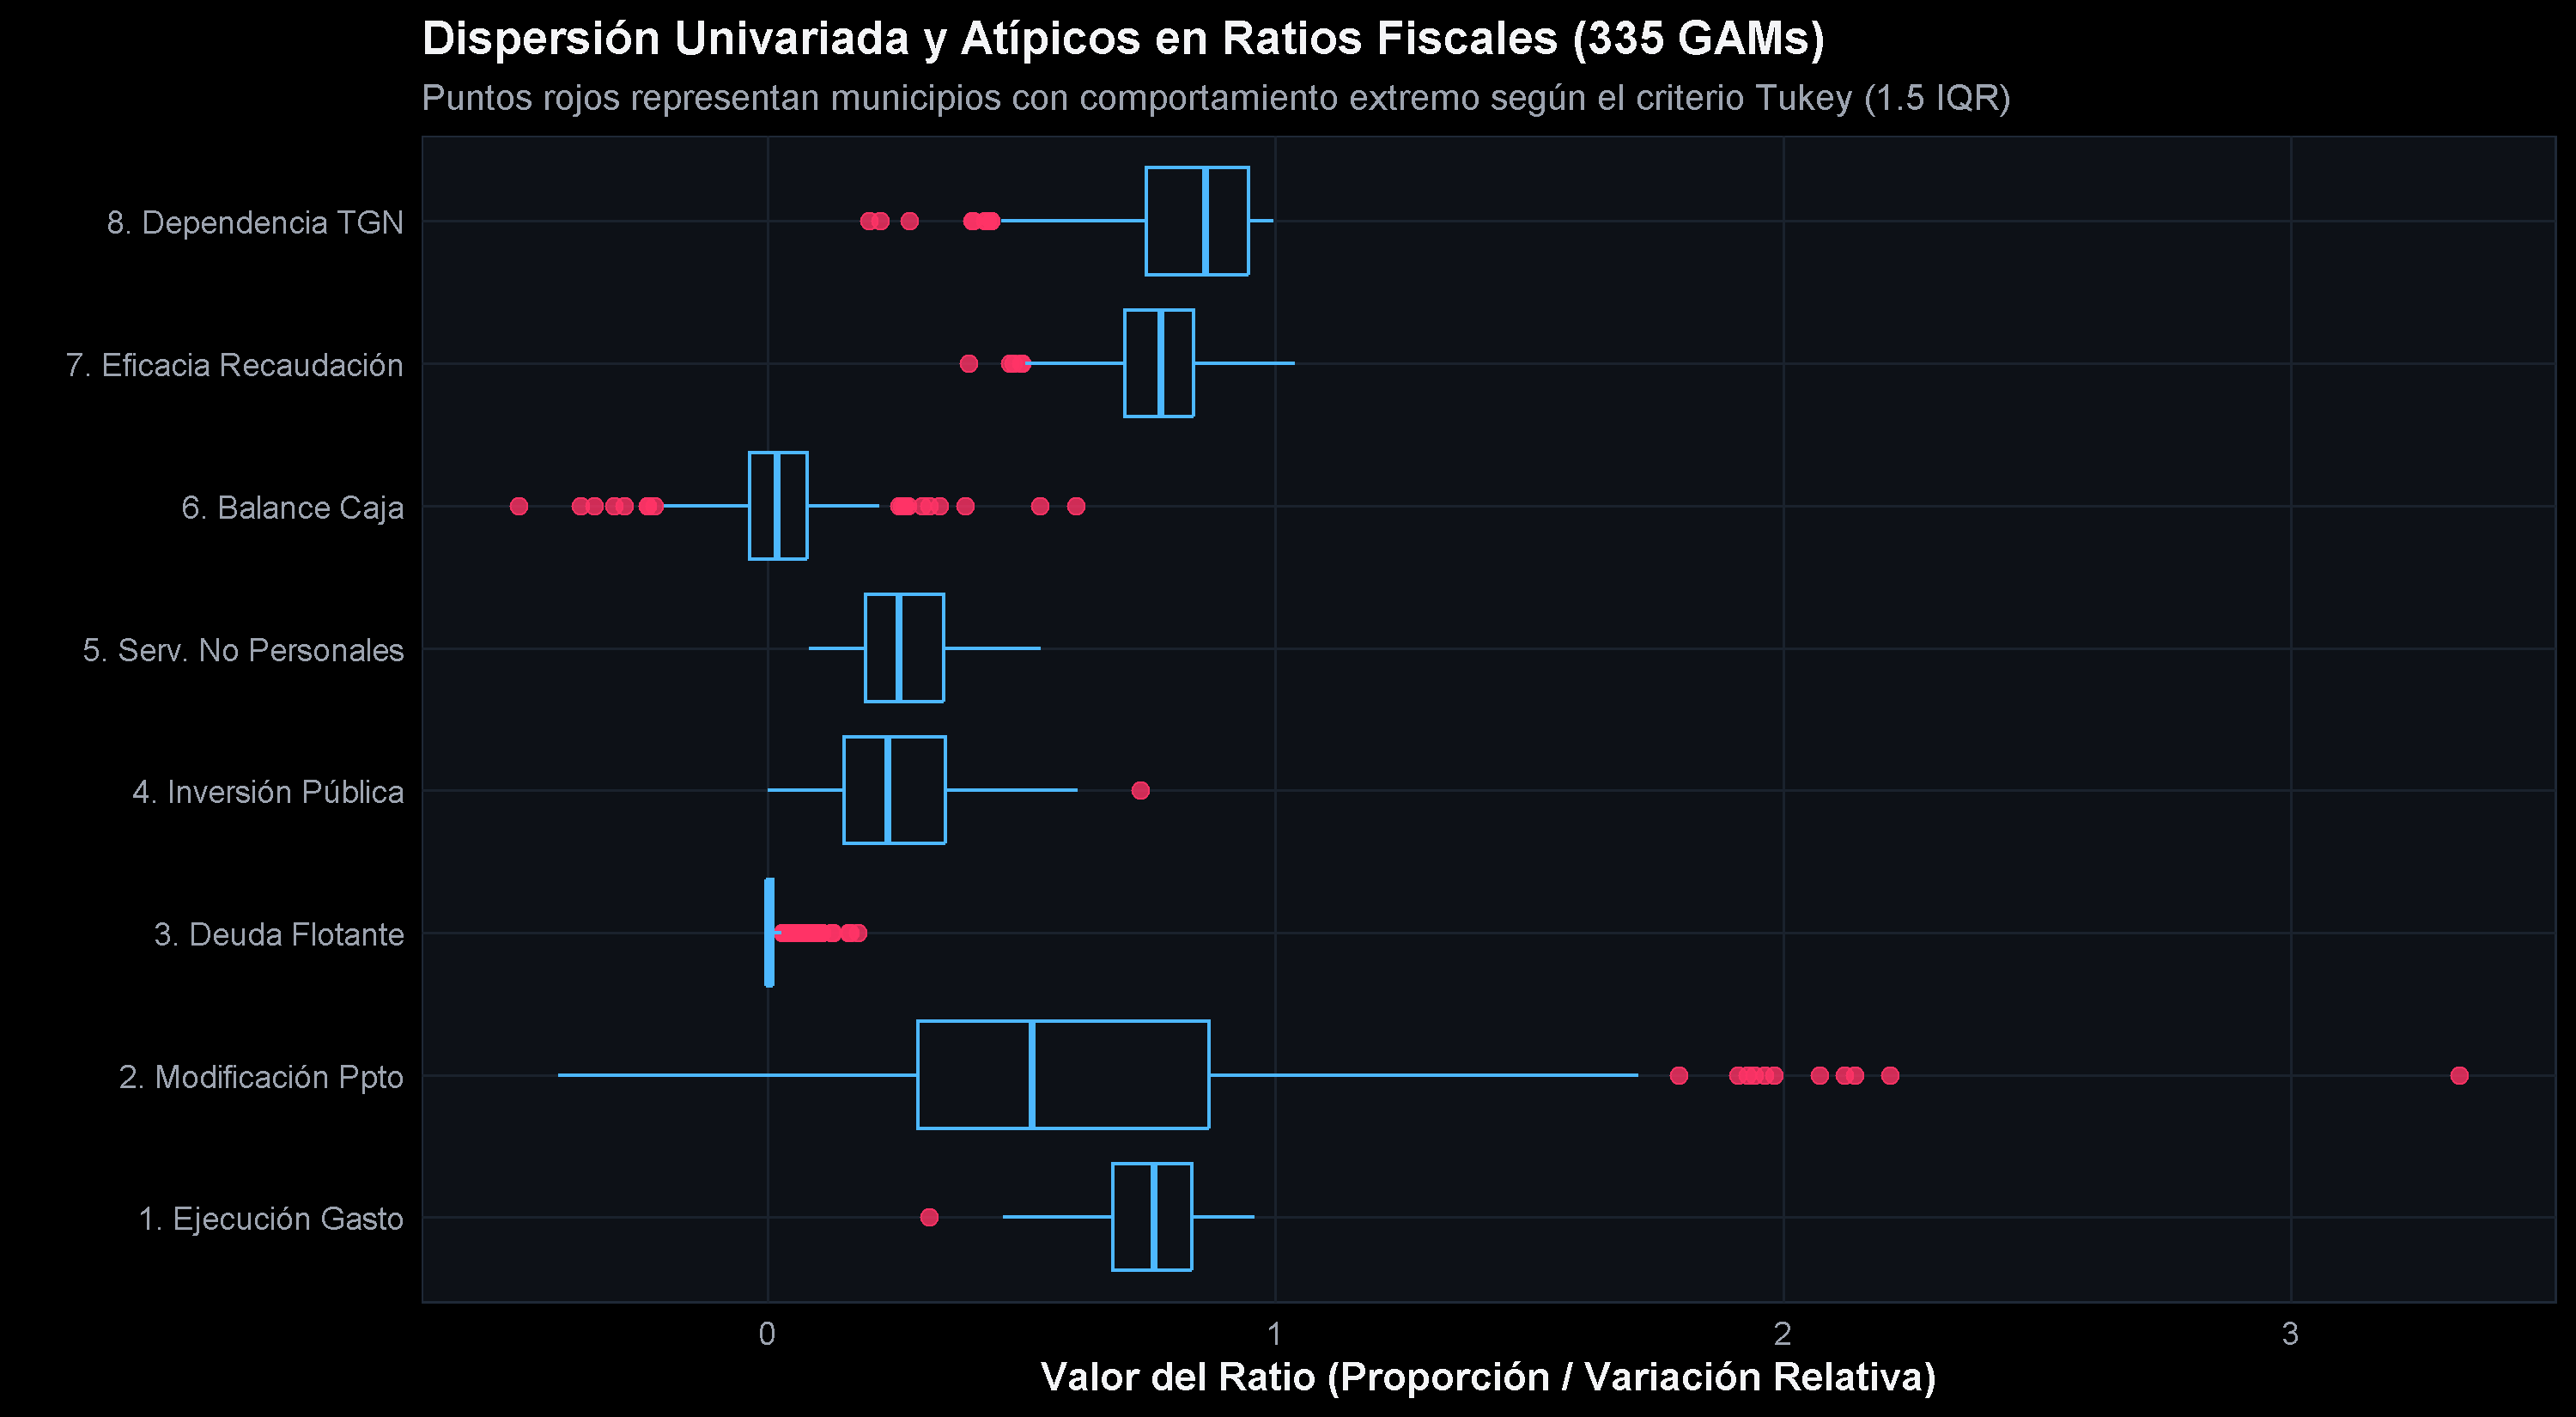
\includegraphics[width=0.92\textwidth]{figuras/fig_02_boxplot_ratios_tukey.png}
    \caption{Distribución y dispersión univariada de los 9 ratios fiscales normalizados (335 GAMs de Bolivia, Gestión 2025).}
    \label{fig:boxplot_ratios}
\end{figure}

\subsection{Segmentación y Regímenes con Mezclas Gaussianas (GMM)}
El algoritmo EM evaluó parametrizaciones geométricas para $G \in \{1, \dots, 9\}$. La maximización del criterio BIC ($\text{BIC} = -5.284,80$) seleccionó como óptimo el modelo \textbf{VVE} (elipsoidal, igual orientación, volumen y forma variable) con exactamente \textbf{$G = 4$ regímenes fiscales} (Figura \ref{fig:gmm_bic}).

\begin{figure}[H]
    \centering
    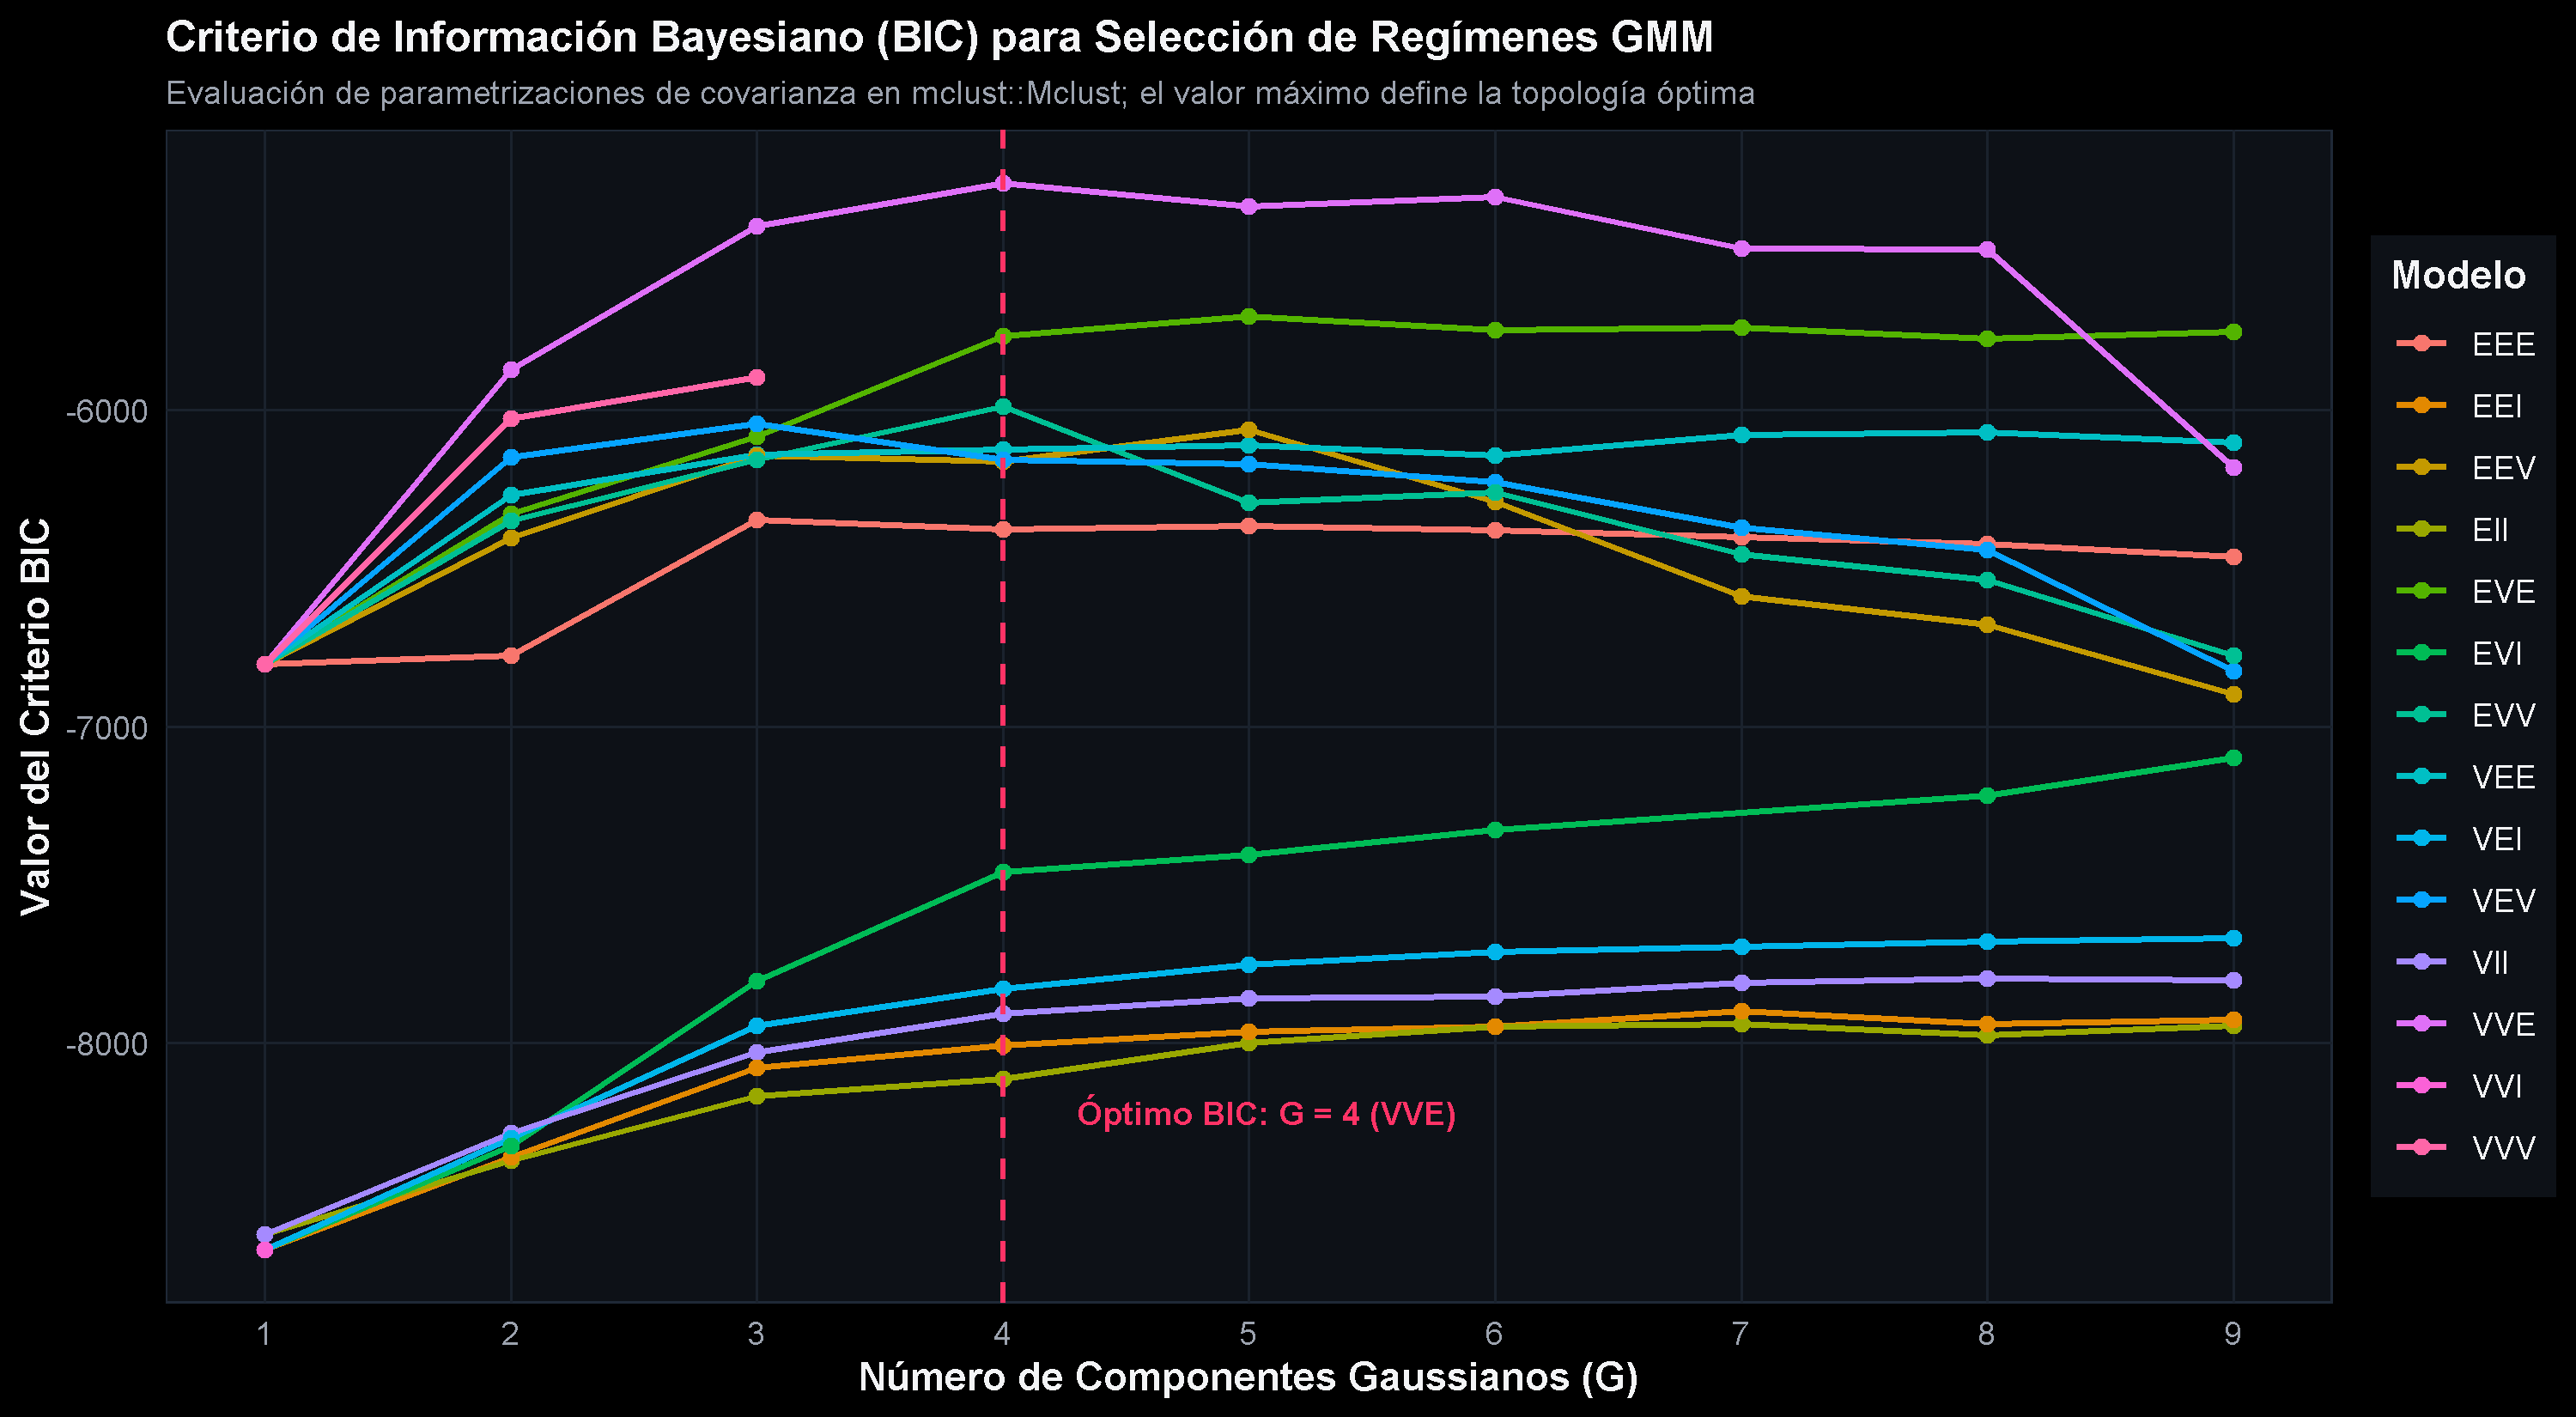
\includegraphics[width=0.88\textwidth]{figuras/fig_03_gmm_curva_bic.png}
    \caption{Curva de selección de modelo por Criterio de Información Bayesiano (BIC) en \texttt{mclust}.}
    \label{fig:gmm_bic}
\end{figure}

La caracterización macroeconómica de los 4 regímenes (Tabla \ref{tab:gmm_regimenes}) refleja la heterogeneidad de los municipios bolivianos:
\begin{itemize}[noitemsep]
    \item \textbf{Régimen 1 (90 GAMs, 26,9\%):} Municipios rurales de alta inversión comunal (28,5\%) y extrema dependencia del TGN (87,9\%).
    \item \textbf{Régimen 2 (94 GAMs, 28,1\%):} Municipios con alta concentración en Servicios No Personales (27,9\%).
    \item \textbf{Régimen 3 (48 GAMs, 14,3\%):} Municipios urbanos e intermedios de mayor escala fiscal (promedio Bs. 200,9M) con ingresos propios tributarios destacados.
    \item \textbf{Régimen 4 (103 GAMs, 30,7\%):} Conglomerado fiscal estándar promedio nacional.
\end{itemize}

\begin{table}[htbp]
\centering
\footnotesize
\caption{Caracterizaci\'on de los Reg\'imenes Fiscales Identificados por el Modelo GMM (VVE, $G=4$)}
\label{tab:gmm_regimenes}
\begin{tabular}{lrrrrrr}
\hline
\textbf{R\'egimen} & \textbf{Tama\~no} & \textbf{Ejec. Gasto} & \textbf{Inversi\'on} & \textbf{Serv. No Pers.} & \textbf{Dep. TGN} & \textbf{Ppto. Prom.} \\
\hline
R\'egimen 1 & 90 (26.9\%) & 70.9\% & 28.5\% & 27.9\% & 87.9\% & Bs. 23.3M \\
R\'egimen 2 & 94 (28.1\%) & 77.4\% & 23.9\% & 27.9\% & 84.3\% & Bs. 31.6M \\
R\'egimen 3 & 48 (14.3\%) & 75.2\% & 23.5\% & 26.4\% & 73.0\% & Bs. 252.9M \\
R\'egimen 4 & 103 (30.7\%) & 76.8\% & 24.4\% & 27.1\% & 80.3\% & Bs. 78.8M \\
\hline
\end{tabular}
\end{table}


El análisis de log-densidad probabilística multivariante identificó 17 municipios por debajo del umbral del 5\% ($\ln p(\mathbf{x}_i) \le -14,526$), categorizados como anomalías globales de baja verosimilitud conjunta.

\subsection{Análisis de Densidad Local con LOF y Sensibilidad Multiescala}
El algoritmo LOF computó la atipicidad respecto al vecindario con parámetro base $minPts = 20$. Con un corte de $\text{LOF} > 1,5$, se detectaron 16 municipios con deterioro severo de densidad local.

\begin{figure}[H]
    \centering
    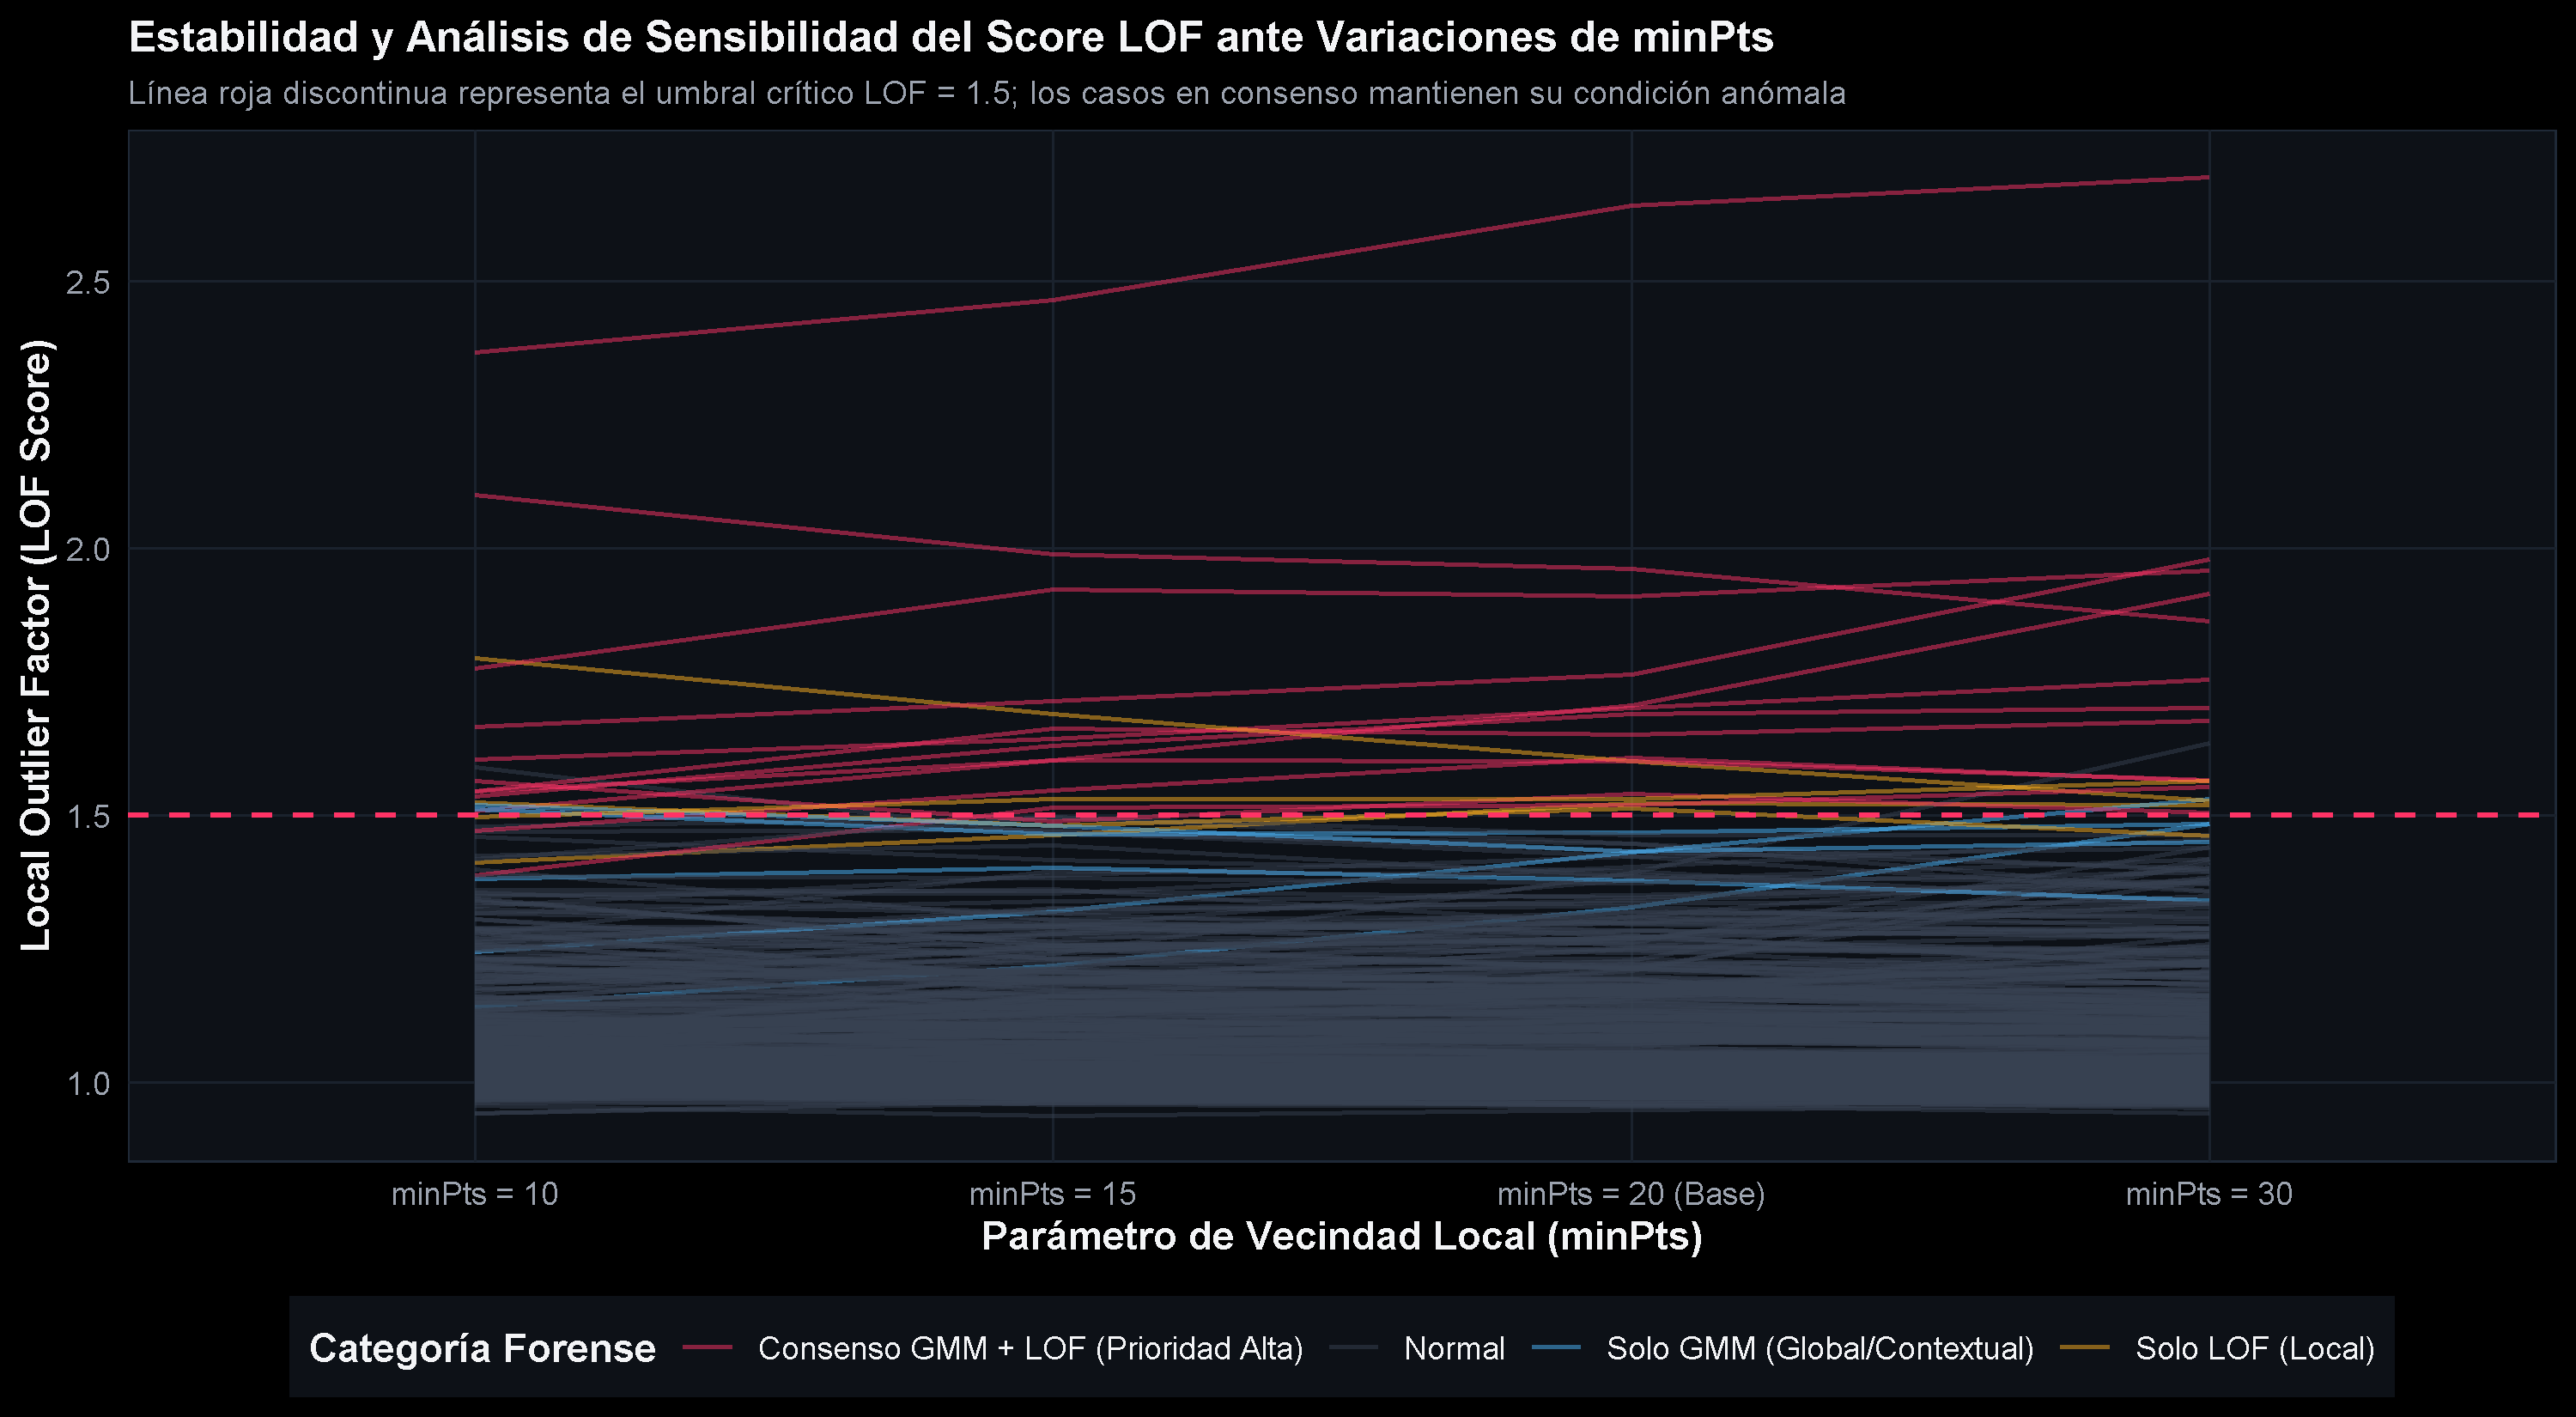
\includegraphics[width=0.88\textwidth]{figuras/fig_05_sensibilidad_lof.png}
    \caption{Evaluación de sensibilidad y estabilidad de los scores LOF para $minPts \in \{10, 15, 20, 30\}$.}
    \label{fig:sensibilidad_lof}
\end{figure}

El análisis de sensibilidad (Figura \ref{fig:sensibilidad_lof}) confirmó la robustez del modelo: la correlación de Pearson entre los diferentes valores de vecindad superó sistemáticamente $0,94$ ($r = 0,987$ entre 15 y 20; $r = 0,978$ entre 20 y 30), demostrando que la condición de atipicidad no es un sesgo del parámetro elegido, sino una propiedad topológica persistente de los datos fiscales.

\subsection{Matriz de Consenso y Proyección PCA}
La triangulación de los dos paradigmas (densidad global paramétrica GMM y densidad local no paramétrica LOF) clasificó a los 335 GAMs en cuatro grupos:
\begin{itemize}[noitemsep]
    \item \textbf{Normales:} 314 municipios (93,73\%).
    \item \textbf{Solo GMM (Global/Contextual):} 5 municipios (1,49\%).
    \item \textbf{Solo LOF (Local):} 4 municipios (1,19\%).
    \item \textbf{Consenso GMM + LOF (Prioridad Alta):} \textbf{12 municipios críticos (3,58\%)}, presentados en la Tabla \ref{tab:consenso_anomalias}.
\end{itemize}

\begin{figure}[H]
    \centering
    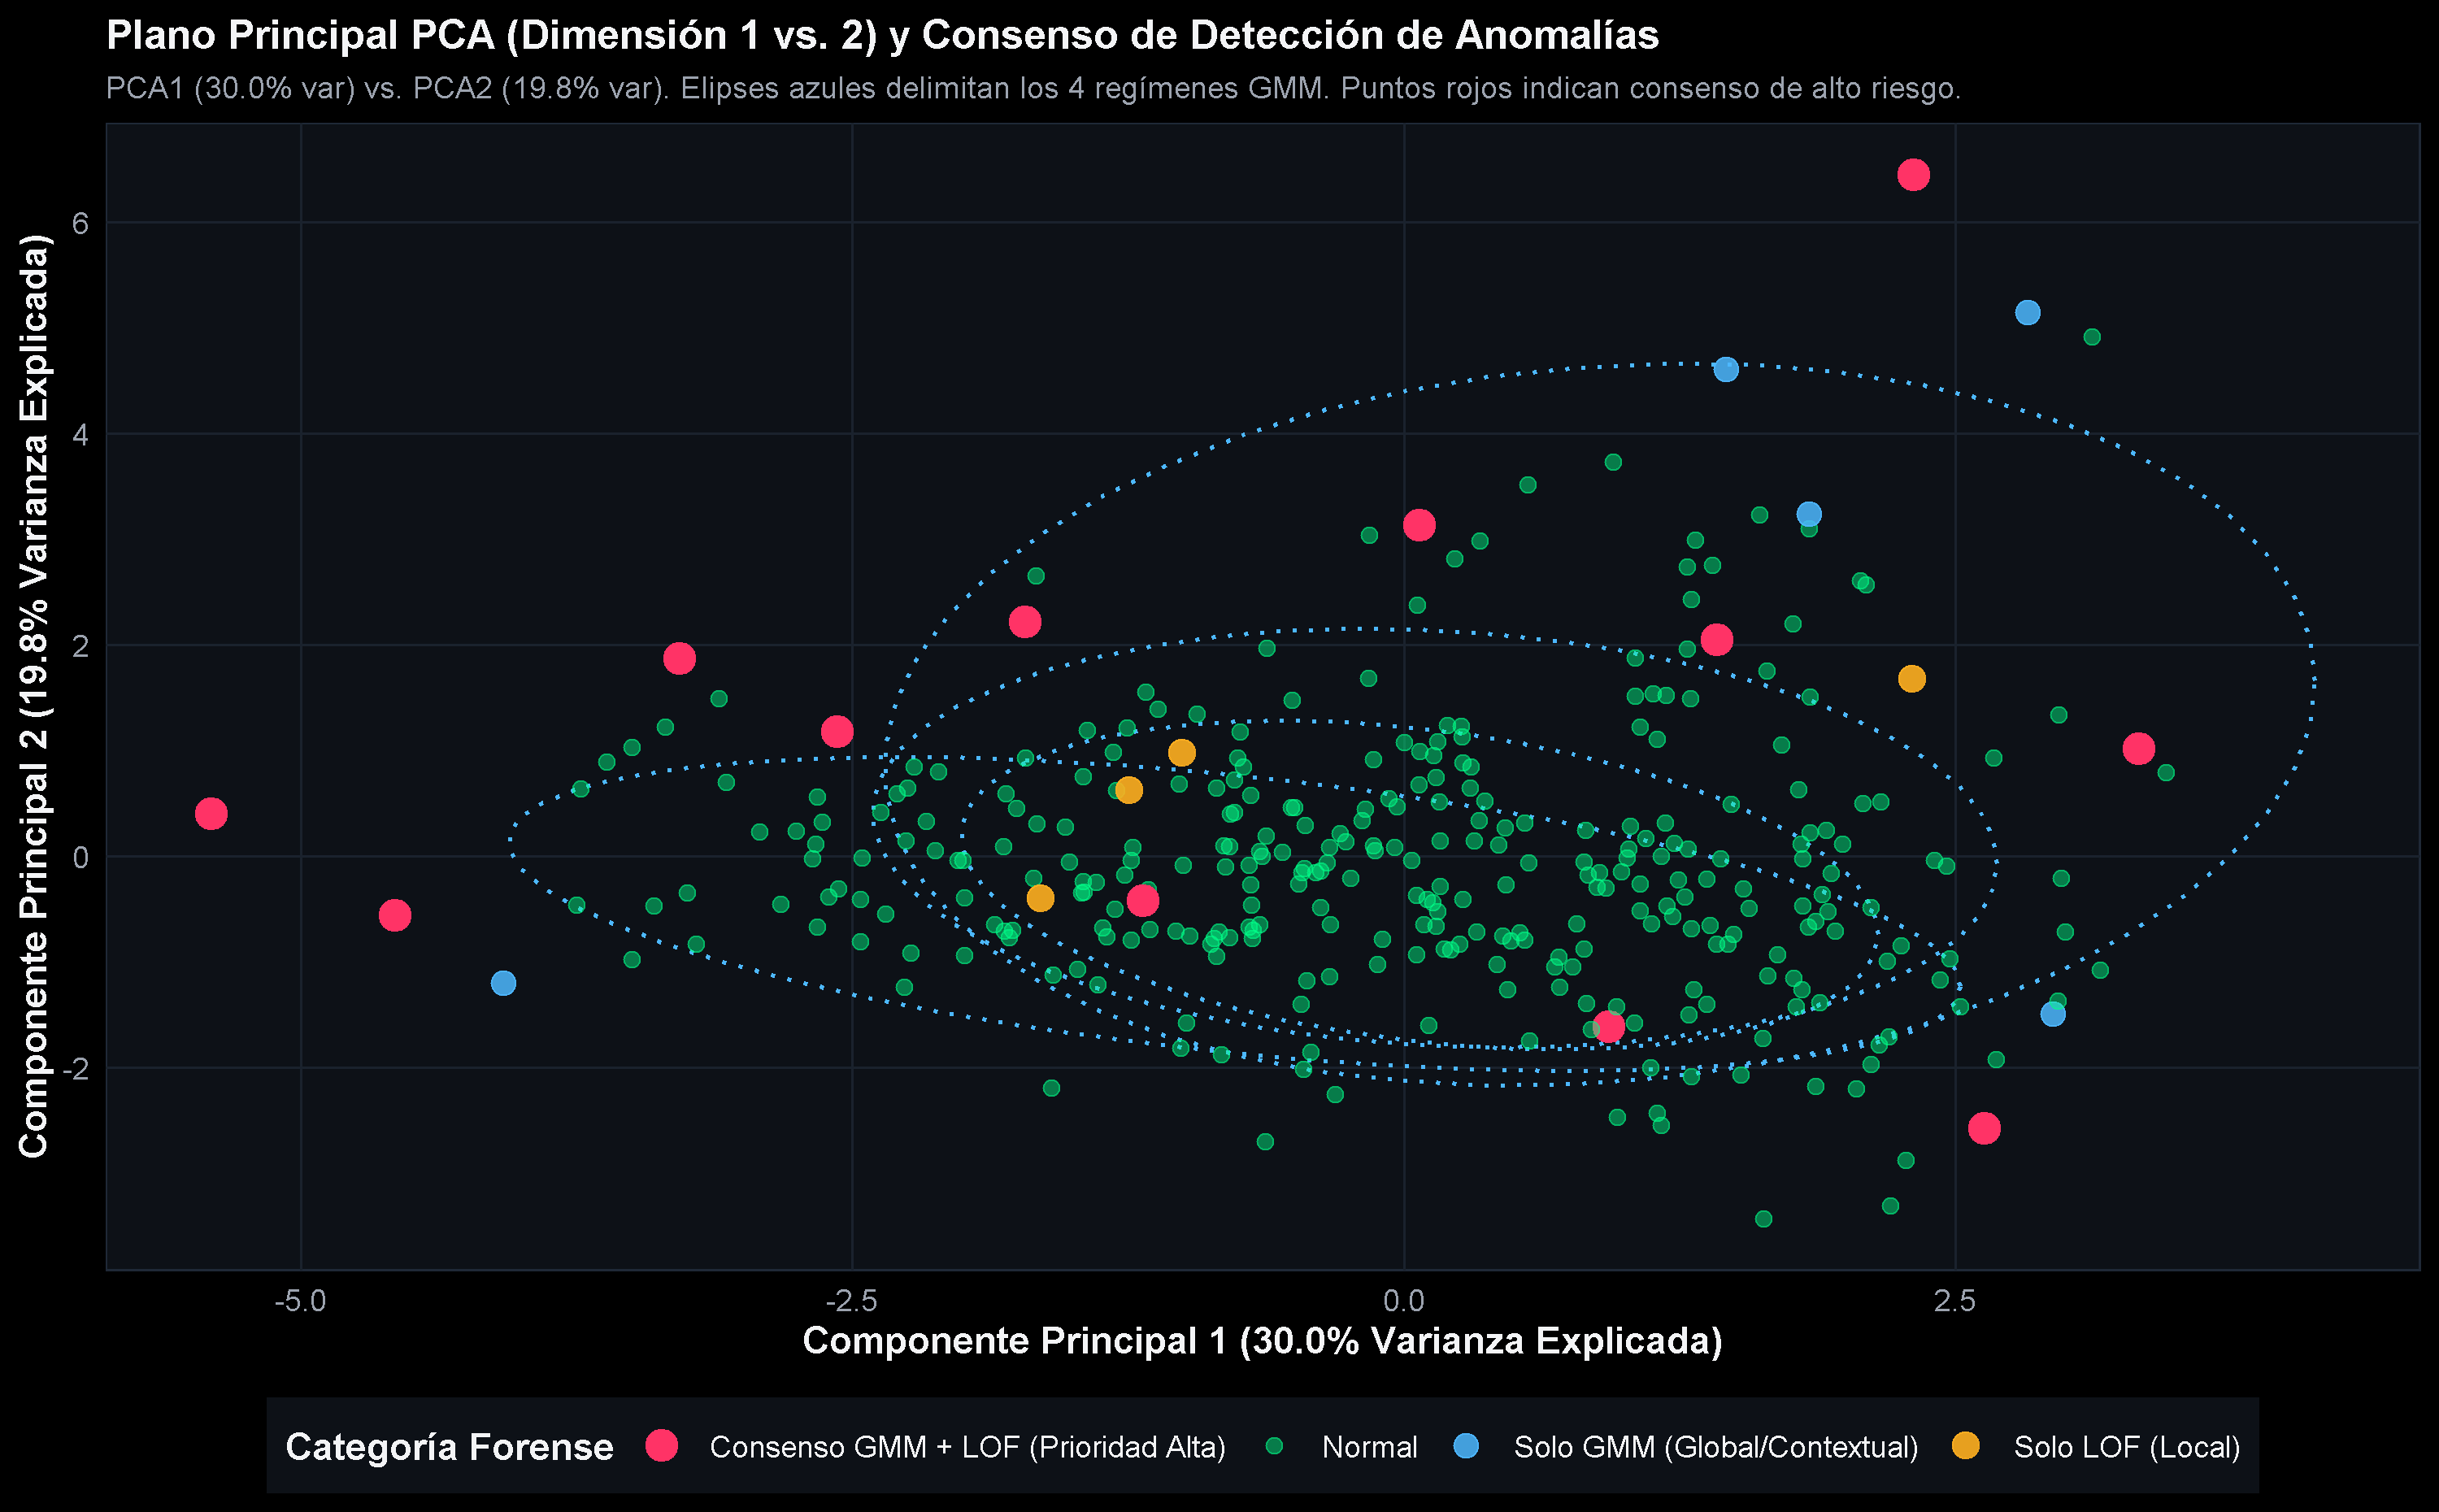
\includegraphics[width=0.94\textwidth]{figuras/fig_04_pca_consenso_anomalias.png}
    \caption{Espacio latente de Componentes Principales (PCA) con elipses de regímenes GMM y ubicación de los 12 municipios priorizados en consenso.}
    \label{fig:pca_consenso}
\end{figure}

\begin{table}[htbp]
\centering
\caption{Municipios Prioritarios en Consenso GMM + LOF (Alta Probabilidad de Anomal\'ia Forense)}
\label{tab:consenso_anomalias}
\resizebox{\textwidth}{!}{%
\begin{tabular}{llrrrrl}
\hline
\textbf{Gobierno Municipal} & \textbf{Depto.} & \textbf{Ejec.} & \textbf{Deuda Flot.} & \textbf{LOF} & \textbf{Log-Dens.} & \textbf{Diagn\'ostico Forense Preliminar} \\
\hline
Gobierno Aut\'onomo Municipal De Chulumani (Villa De La Libertad) & LA PAZ & 31.9\% & 16.20\% & 2.64 & -20.2 & Par\'alisis fiscal y acumulaci\'on inercial \\
Gobierno Aut\'onomo Municipal De Mojinete & POTOSI & 78.7\% & 0.82\% & 1.96 & -25.0 & D\'eficit cr\'itico de tesorer\'ia \\
Gobierno Aut\'onomo Municipal De Tahua & POTOSI & 46.3\% & 2.45\% & 1.91 & -22.7 & Gasto corriente total (Cero inversi\'on) \\
Gobierno Aut\'onomo Municipal De Santa Cruz De La Sierra & SANTA CRUZ & 80.0\% & 17.77\% & 1.76 & -20.2 & Severa deuda flotante e iliquidez \\
Gobierno Aut\'onomo Municipal De Caquiaviri & LA PAZ & 89.1\% & 15.95\% & 1.70 & -17.0 & Severa deuda flotante e iliquidez \\
Gobierno Aut\'onomo Municipal De Humanata & LA PAZ & 55.0\% & 0.04\% & 1.70 & -17.6 & Gasto at\'ipico concentrado en inversi\'on \\
Gobierno Aut\'onomo Municipal De San Juan & SANTA CRUZ & 49.3\% & 1.53\% & 1.69 & -18.5 & Distorsi\'on multivariante combinada \\
Gobierno Aut\'onomo Municipal De Antequera & ORURO & 67.0\% & 0.00\% & 1.65 & -19.2 & D\'eficit cr\'itico de tesorer\'ia \\
Gobierno Aut\'onomo Municipal De Malla & LA PAZ & 65.8\% & 8.34\% & 1.61 & -16.2 & Gasto at\'ipico concentrado en inversi\'on \\
Gobierno Aut\'onomo Municipal De Colpa B\'elgica & SANTA CRUZ & 89.1\% & 0.04\% & 1.60 & -15.8 & Distorsi\'on multivariante combinada \\
Gobierno Aut\'onomo Municipal De Boyuibe & SANTA CRUZ & 65.0\% & 7.14\% & 1.54 & -16.2 & Distorsi\'on multivariante combinada \\
Gobierno Aut\'onomo Municipal De Colcha ``K'' (Villa Mart\'in) & POTOSI & 68.1\% & 0.00\% & 1.52 & -15.2 & Distorsi\'on multivariante combinada \\
\hline
\end{tabular}%
}
\end{table}


La proyección en componentes principales (Figura \ref{fig:pca_consenso}) captura el 48,7\% de la varianza total acumulada en los dos primeros ejes (PC1: 27,4\%, PC2: 21,3\%). Los vectores de carga (*loadings*) revelan que PC1 está dominado por la escala presupuestaria y la deuda flotante en sentido positivo, mientras que PC2 separa a los municipios según su balance de caja y nivel de inversión pública.

\subsection{Análisis Metodológico de Anomalías Unilaterales}
El estudio de los casos no coincidentes ofrece un alto valor epistemológico:
\begin{itemize}[noitemsep]
    \item \textbf{Solo GMM (5 municipios):} Corresponden a observaciones ubicadas en las fronteras exteriores de las elipses gaussianas. Tienen valores moderadamente inusuales en varias dimensiones a la vez, lo que disminuye su log-densidad global, pero se encuentran rodeados de vecinos a distancias homogéneas, por lo que su LOF se mantiene por debajo de 1,5.
    \item \textbf{Solo LOF (4 municipios):} Representan anomalías de densidad local. Se sitúan en zonas con densidades globales intermedias, pero están relativamente aislados de sus vecinos inmediatos más cercanos en subespacios específicos de gasto corriente y transferencias.
\end{itemize}

% ------------------------------------------------------------------------------
\section{Auditoría Forense Drill-Down y Expedientes Críticos}
% ------------------------------------------------------------------------------
Sobre los 12 municipios identificados en consenso, se realizó una extracción en profundidad de sus 6.387 transacciones crudas de gasto devengado para ejecutar pruebas de microdatos contables.

\subsection{Conformidad con la Ley de Benford}
La Tabla \ref{tab:auditoria_benford} expone los resultados de la prueba del primer dígito de Benford. De acuerdo a los umbrales de \citet{nigrini2012benford}, cinco municipios caen en la categoría de \textbf{No Conformidad ($\text{MAD} > 0,015$)}: Caquiaviri, Tahua, Chulumani, Antequera y San Juan.

\begin{table}[htbp]
\centering
\caption{Resultados de la Prueba de Conformidad con la Ley de Benford y Duplicados Exactos}
\label{tab:auditoria_benford}
\resizebox{\textwidth}{!}{%
\begin{tabular}{llrrrrrr}
\hline
\textbf{Gobierno Municipal} & \textbf{Depto.} & \textbf{Partidas} & \textbf{MAD} & \textbf{Conformidad (Nigrini)} & \textbf{Chi-Cuad.} & \textbf{p-valor} & \textbf{Duplicados} \\
\hline
Gobierno Autónomo Municipal De Chulumani (Villa De La Libertad) & LA PAZ & 138 & 0.0170 & Nonconformity & 9.35 & 0.3139 & 2.9\% \\
Gobierno Autónomo Municipal De Mojinete & POTOSI & 196 & 0.0136 & Marginally acceptable conformity & 4.42 & 0.8173 & 12.8\% \\
Gobierno Autónomo Municipal De Tahua & POTOSI & 76 & 0.0212 & Nonconformity & 5.47 & 0.7062 & 9.2\% \\
Gobierno Autónomo Municipal De Santa Cruz De La Sierra & SANTA CRUZ & 2830 & 0.0054 & Close conformity & 8.42 & 0.3936 & 6.8\% \\
Gobierno Autónomo Municipal De Caquiaviri & LA PAZ & 239 & 0.0241 & Nonconformity & 16.91 & 0.0311 & 9.2\% \\
Gobierno Autónomo Municipal De Humanata & LA PAZ & 229 & 0.0143 & Marginally acceptable conformity & 6.45 & 0.5971 & 10.5\% \\
Gobierno Autónomo Municipal De San Juan & SANTA CRUZ & 219 & 0.0160 & Nonconformity & 11.39 & 0.1807 & 14.2\% \\
Gobierno Autónomo Municipal De Antequera & ORURO & 382 & 0.0165 & Nonconformity & 12.11 & 0.1465 & 8.4\% \\
Gobierno Autónomo Municipal De Malla & LA PAZ & 385 & 0.0095 & Acceptable conformity & 3.62 & 0.8894 & 10.9\% \\
Gobierno Autónomo Municipal De Colpa Bélgica & SANTA CRUZ & 409 & 0.0121 & Marginally acceptable conformity & 10.36 & 0.2409 & 7.8\% \\
Gobierno Autónomo Municipal De Boyuibe & SANTA CRUZ & 690 & 0.0080 & Acceptable conformity & 7.60 & 0.4737 & 19.9\% \\
Gobierno Autónomo Municipal De Colcha"K" (Villa Martín) & POTOSI & 594 & 0.0114 & Acceptable conformity & 8.73 & 0.3655 & 15.3\% \\
\hline
\end{tabular}%
}
\end{table}


El caso más destacado es el \textbf{GAM de Caquiaviri (La Paz)} (Figura \ref{fig:benford_caq}): con 239 partidas devengadas, registra una desviación estadísticamente significativa ($\chi^2 = 16,91$, $p = 0,031 < 0,05$, $\text{MAD} = 0,0241$). La distribución observada exhibe una supresión anormal del dígito 1 (21,3\% observado frente al 30,1\% teórico) y picos desproporcionados en los dígitos 4 y 5, descartando aleatoriedad con una confianza del 96,9\%.

\begin{figure}[H]
    \centering
    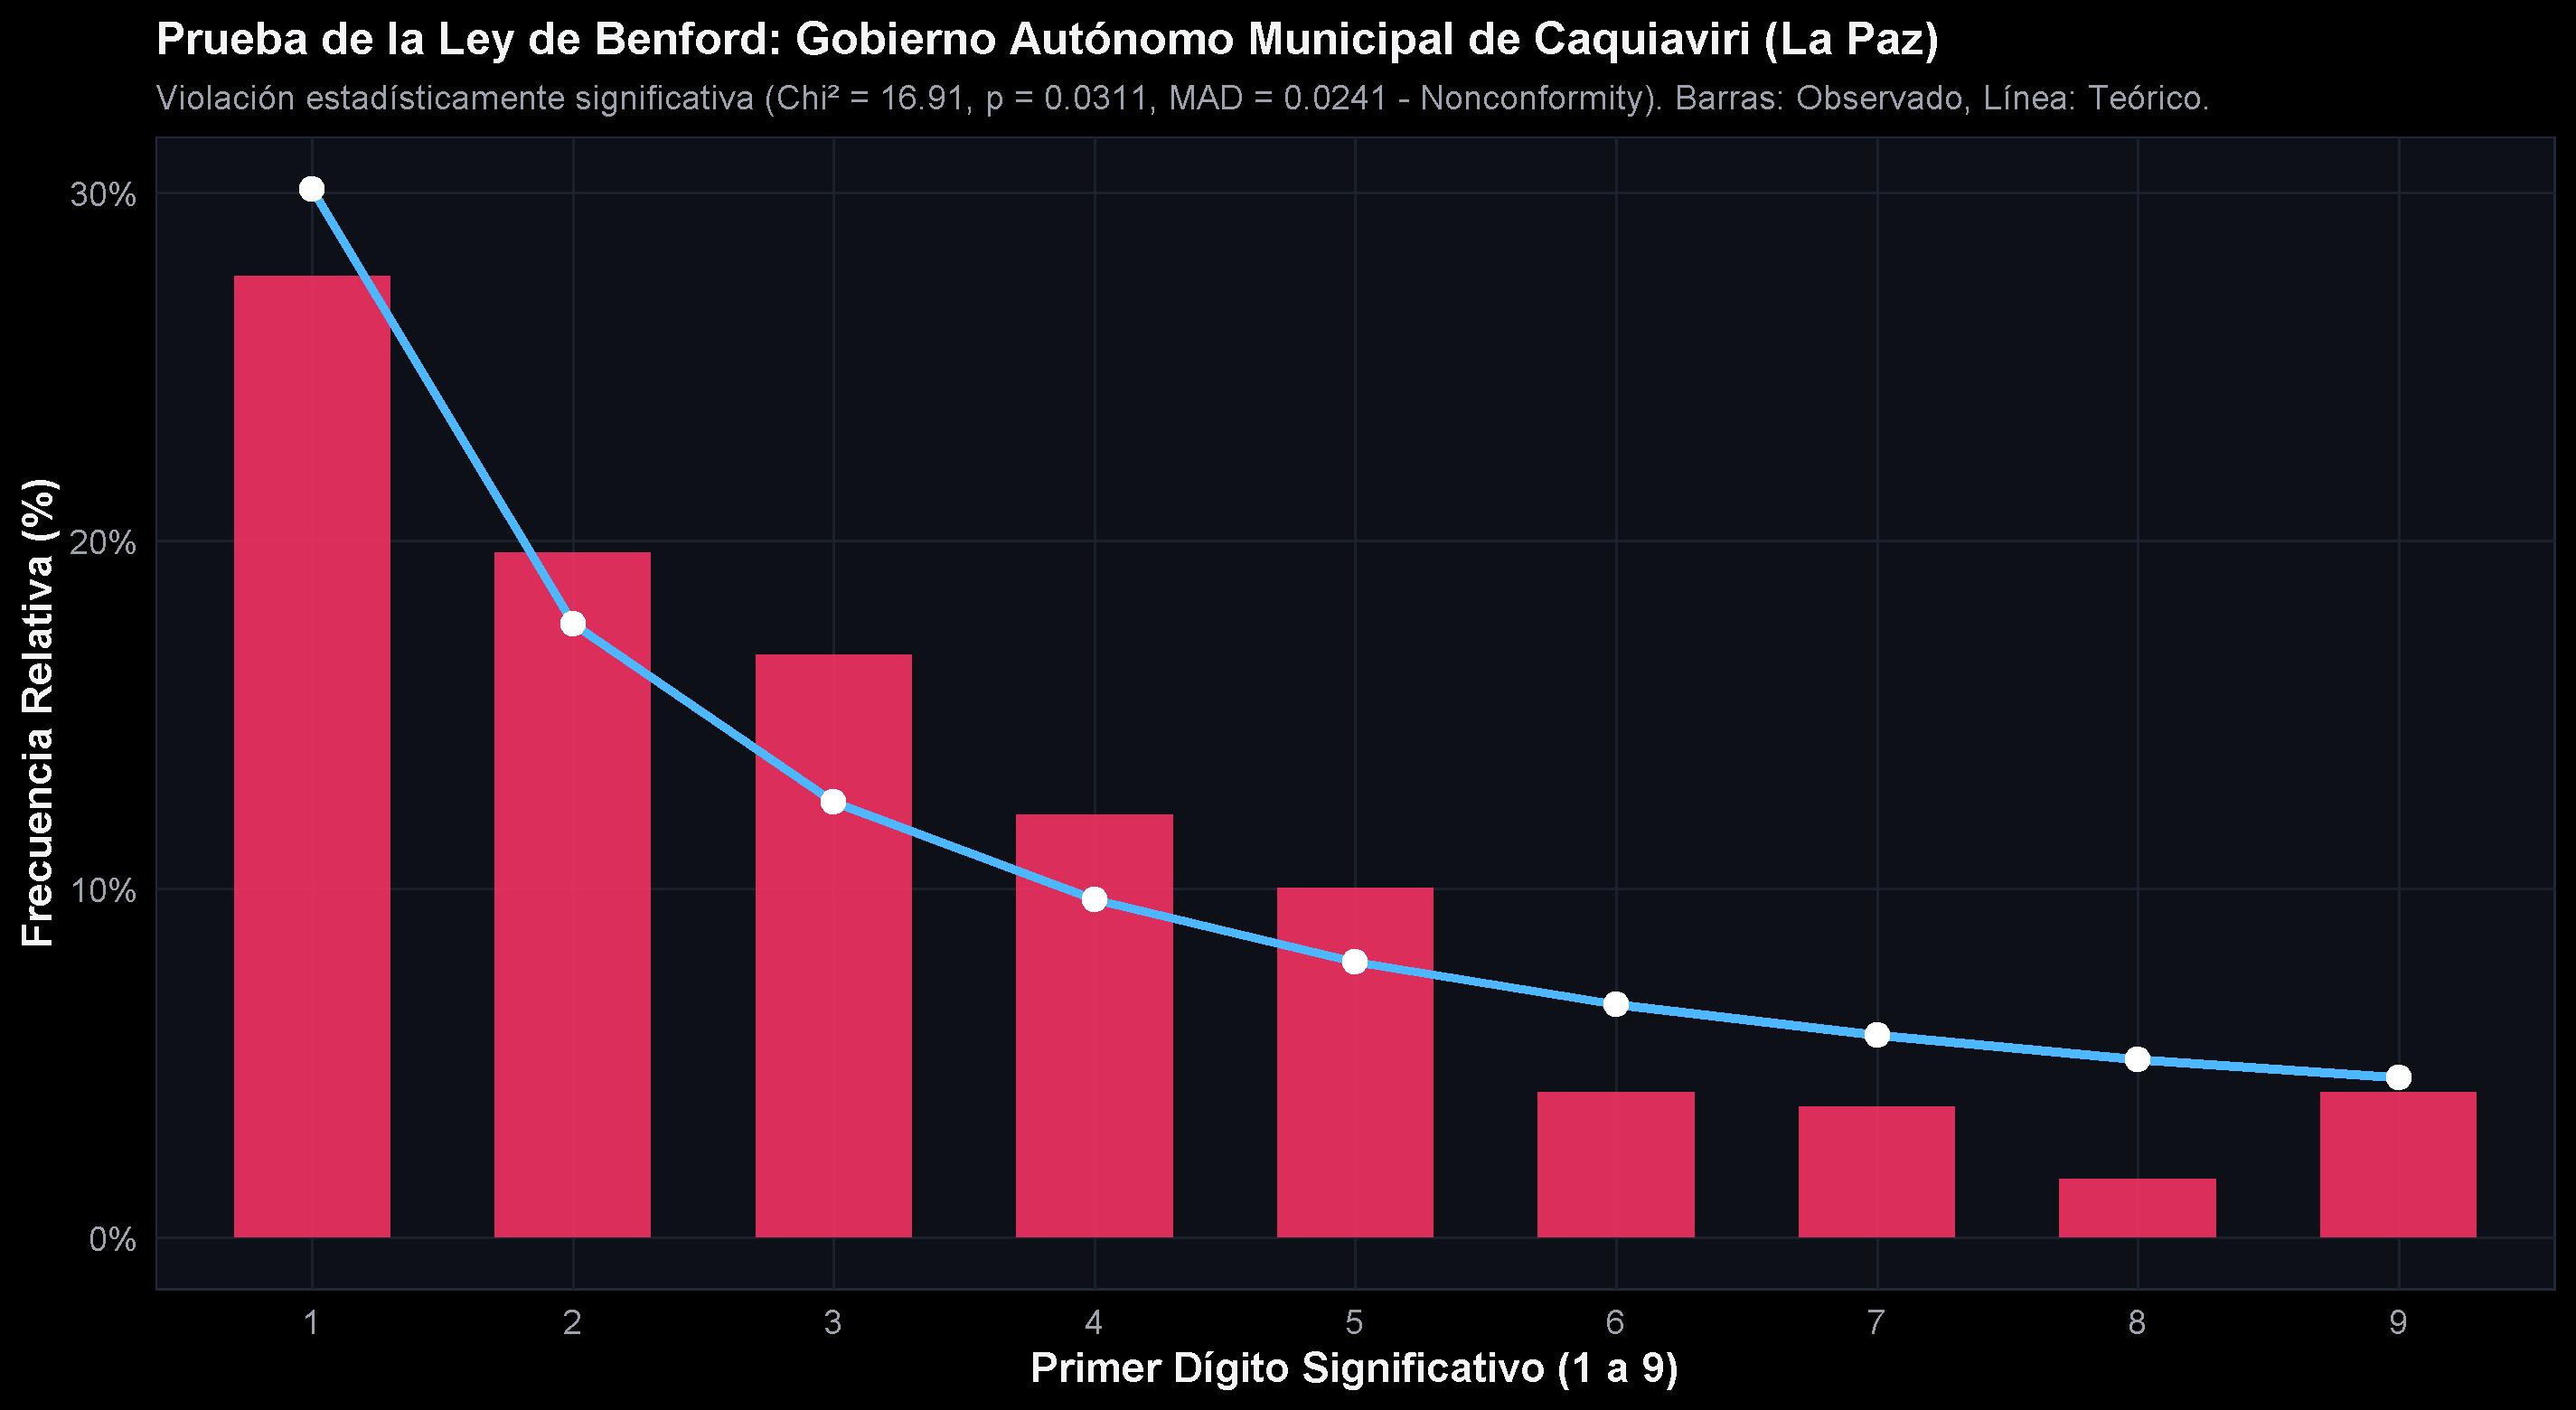
\includegraphics[width=0.88\textwidth]{figuras/fig_06_benford_caquiaviri.png}
    \caption{Prueba de la Ley de Benford en Caquiaviri: discrepancia empírica estadísticamente significativa ($p = 0,031$).}
    \label{fig:benford_caq}
\end{figure}

\subsection{Fraccionamiento de Contratos y Montos Duplicados (D.S. 0181)}
La inspección transaccional identificó una fuerte concentración de comprobantes emitidos por montos monetarios idénticos y repetitivos (Tabla \ref{tab:duplicados_sospechosos}):
\begin{itemize}[noitemsep]
    \item \textbf{GAM de Boyuibe (Santa Cruz):} El \textbf{19,86\%} de todas sus partidas devengadas (137 de 690 comprobantes) corresponde a cifras repetidas, destacando múltiples adquisiciones de Bs. 20.000 y Bs. 50.000 en insumos y servicios.
    \item \textbf{GAM de Colcha ``K'' (Potosí):} A pesar de administrar un presupuesto de Bs. 127 millones por regalías mineras, el \textbf{15,32\%} de sus registros son montos idénticos reiterativos de Bs. 20.000, Bs. 48.000 y Bs. 50.000.
    \item \textbf{GAM de San Juan (Santa Cruz):} Concentra un \textbf{14,16\%} de transacciones duplicadas.
\end{itemize}

\begin{table}[htbp]
\centering
\caption{Top 10 Casos de Montos Id\'enticos Reincidentes (Alerta Forense de Posible Fraccionamiento)}
\label{tab:duplicados_sospechosos}
\resizebox{\textwidth}{!}{%
\begin{tabular}{llrrr}
\hline
\textbf{Gobierno Municipal} & \textbf{Depto.} & \textbf{Monto Repetido} & \textbf{Repeticiones} & \textbf{Monto Total Acum.} \\
\hline
Gobierno Autónomo Municipal De Santa Cruz De La Sierra & SANTA CRUZ & Bs. 20.000 & 16 & Bs. 320.000 \\
Gobierno Autónomo Municipal De Colcha"K" (Villa Martín) & POTOSI & Bs. 20.000 & 9 & Bs. 180.000 \\
Gobierno Autónomo Municipal De Colcha"K" (Villa Martín) & POTOSI & Bs. 10.000 & 9 & Bs. 90.000 \\
Gobierno Autónomo Municipal De Colcha"K" (Villa Martín) & POTOSI & Bs. 15.000 & 8 & Bs. 120.000 \\
Gobierno Autónomo Municipal De Santa Cruz De La Sierra & SANTA CRUZ & Bs. 22.000 & 7 & Bs. 154.000 \\
Gobierno Autónomo Municipal De Colcha"K" (Villa Martín) & POTOSI & Bs. 30.000 & 6 & Bs. 180.000 \\
Gobierno Autónomo Municipal De Caquiaviri & LA PAZ & Bs. 20.000 & 6 & Bs. 120.000 \\
Gobierno Autónomo Municipal De San Juan & SANTA CRUZ & Bs. 50.000 & 5 & Bs. 250.000 \\
Gobierno Autónomo Municipal De Santa Cruz De La Sierra & SANTA CRUZ & Bs. 40.000 & 5 & Bs. 200.000 \\
Gobierno Autónomo Municipal De Santa Cruz De La Sierra & SANTA CRUZ & Bs. 36.000 & 5 & Bs. 180.000 \\
\hline
\end{tabular}%
}
\end{table}


Bajo el D.S. N° 0181, los límites de contratación menor se establecen habitualmente en Bs. 20.000 y Bs. 50.000. La emisión repetitiva de facturas y órdenes justo al borde de dichos topes constituye una señal de alerta de fraccionamiento premeditado de compras para eludir convocatorias públicas competitivas.

\begin{figure}[H]
    \centering
    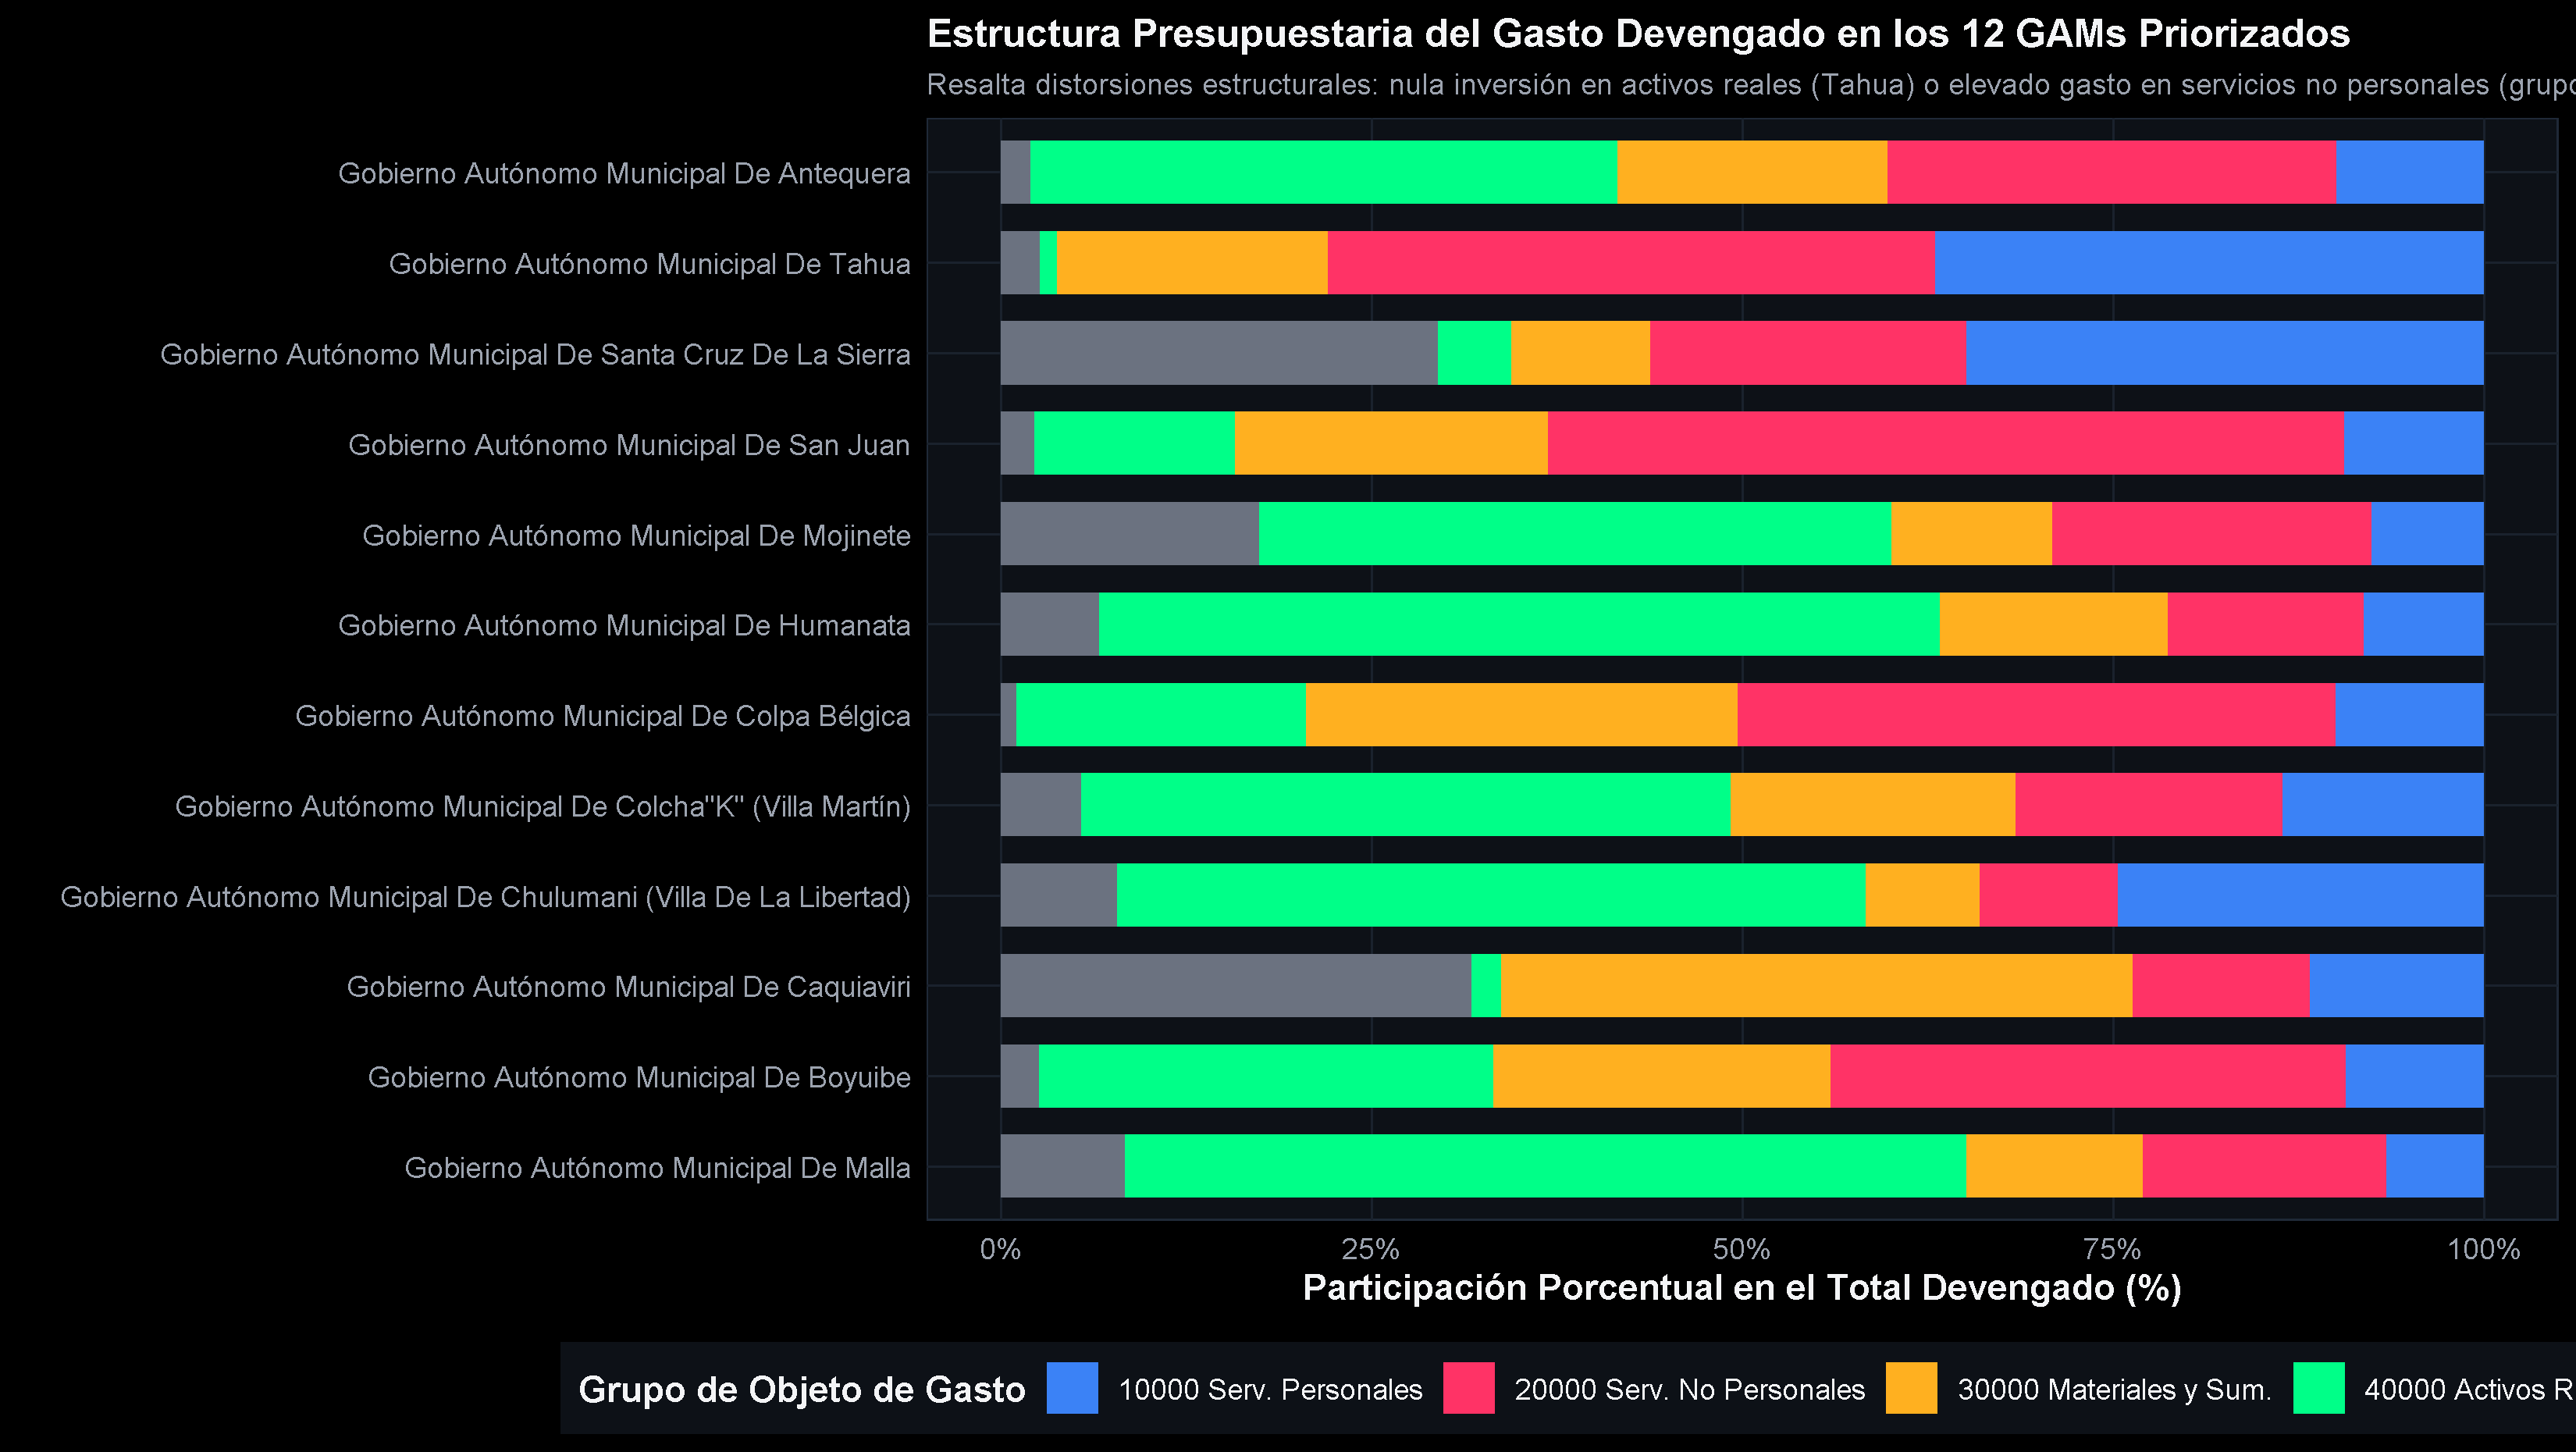
\includegraphics[width=0.94\textwidth]{figuras/fig_07_composicion_gasto_consenso.png}
    \caption{Estructura presupuestaria del gasto devengado por objeto del gasto en los 12 GAMs en consenso.}
    \label{fig:comp_gasto}
\end{figure}

\subsection{Descomposición por Objeto del Gasto y Diagnóstico de Casos}
La Figura \ref{fig:comp_gasto} desglosa la participación por objeto de gasto de los municipios en consenso, permitiendo individualizar las causas de atipicidad:
\begin{enumerate}[label=\textbf{\alph*)}]
    \item \textbf{Tahua (Potosí):} Presenta una patología presupuestaria extrema con un \textbf{0\% de ejecución en Activos Reales} (Grupo 40000). La totalidad de sus recursos se consumió en partidas corrientes de sueldos y materiales.
    \item \textbf{Chulumani (La Paz):} Registra la ejecución de gasto más baja del país (31,87\%) combinada con un balance de caja positivo del +60,78\% y una deuda flotante del 16,20\%. Refleja parálisis de obras con recursos ociosos en tesorería.
    \item \textbf{Santa Cruz de la Sierra:} Presenta la mayor deuda flotante de Bolivia (17,77\%, equivalente a más de Bs. 647 millones impagos a contratistas) y un balance de caja negativo (-2,44\%).
    \item \textbf{Mojinete (Potosí) y Antequera (Oruro):} Presentan balances de caja negativos extremos (-48,98\% y -34,13\% respectivamente), comprometiendo pagos por encima de los ingresos efectivamente recaudados en el año.
    \item \textbf{Humanata y Malla (La Paz):} Exhiben estructuras presupuestarias atípicas con alta concentración en proyectos específicos no recurrentes y brechas significativas entre el presupuesto devengado y pagado.
    \item \textbf{Colpa Bélgica (Santa Cruz):} Muestra una combinación de alta ejecución (89,1\%) con distorsiones multivariantes en servicios no personales y gasto corriente.
\end{enumerate}

\subsection{Matriz de Riesgo Normativo y Responsabilidad (Ley 1178)}
Con base en los hallazgos analíticos, se estructuró una matriz de tipificación de riesgos conforme al régimen de responsabilidades por la función pública de la Ley SAFCO (Tabla \ref{tab:matriz_riesgos_safco}).

\begin{table}[htbp]
\centering
\small
\caption{Matriz de Tipologías de Riesgo Fiscal y Responsabilidad Legal (Ley 1178 y D.S. 0181)}
\label{tab:matriz_riesgos_safco}
\begin{tabularx}{\textwidth}{p{3.2cm}p{4.2cm}p{3.5cm}X}
\hline
\textbf{Tipología de Riesgo} & \textbf{Evidencia Analítica / Métrica} & \textbf{Municipios Ejemplares} & \textbf{Responsabilidad Sugerida (Ley 1178)} \\
\hline
\textbf{Riesgo I: Fraccionamiento Contractual} & Reincidencia de montos idénticos al tope de contratación menor (Bs. 20k / 50k). & Boyuibe (19,9\%), Colcha ``K'' (15,3\%), San Juan (14,2\%) & \textbf{Administrativa y Penal} (Incumplimiento de deberes, D.S. 0181). \\
\textbf{Riesgo II: Parálisis de Inversión y Fondos Ociosos} & Ejecución $< 40\%$, $0\%$ inversión en activos reales y liquidez retenida $> 50\%$. & Chulumani (31,9\% ejec.), Tahua (0\% activos reales) & \textbf{Ejecutiva y Administrativa} (Gestión deficiente o negligente). \\
\textbf{Riesgo III: Iliquidez y Sobreendeudamiento} & Deuda flotante $> 15\%$ y balance de caja negativo en tesorería. & Santa Cruz de la Sierra (17,8\%), Caquiaviri (16,0\%), Mojinete & \textbf{Civil y Ejecutiva} (Compromiso de fondos sin respaldo presupuestario). \\
\textbf{Riesgo IV: Manipulación Documental} & No conformidad severa con Ley de Benford ($p < 0,05$, $\text{MAD} > 0,015$). & Caquiaviri ($p=0,031$, $\text{MAD}=0,024$) & \textbf{Civil y Penal} (Falsedad ideológica o alteración contable). \\
\hline
\end{tabularx}
\end{table}

% ------------------------------------------------------------------------------
\section{Plataforma Interactiva de Monitoreo (Dashboard R Shiny)}
% ------------------------------------------------------------------------------

\subsection{Arquitectura del Sistema y Tecnologías Empleadas}
Para facilitar la transferencia tecnológica hacia los auditores y tomadores de decisión, se implementó y desplegó en la nube una plataforma web interactiva en \textbf{R Shiny} accesible públicamente en \url{https://gmm-lof-deteccion-anomalias-auditoria.onrender.com/} \citep{render_dashboard}, empaquetada mediante contenedorización Docker (\texttt{Dockerfile}) y versionada en GitHub \citep{github_proyecto}. La arquitectura técnica local y de despliegue se apoya en:
\begin{itemize}[noitemsep]
    \item \textbf{Bootstrap 5 y \texttt{bslib}:} Estructura responsiva de diseño ergonómico bajo la filosofía visual \textit{Dark Telemetry} implementada en \texttt{dashboard/www/custom.css}.
    \item \textbf{\texttt{plotly}:} Gráficos interactivos de dispersión, proyecciones 2D y 3D en componentes principales con renderizado WebGL, tooltips y elipses probabilísticas.
    \item \textbf{\texttt{DT}:} Tablas interactivas con capacidad de búsqueda instantánea, paginación, filtros por columnas y botones de exportación a formatos abiertos (CSV, Excel, PDF).
\end{itemize}

\subsection{Estructura Operativa y Módulos del Dashboard}
La plataforma interactiva está organizada en ocho módulos funcionales especializados que cubren desde el análisis macroeconómico hasta el drill-down forense transaccional, accesibles a través de su barra de navegación lateral y superior:

\subsubsection{Pestaña 1: Panorama Fiscal 2025}
La primera pestaña (Figura \ref{fig:dashboard_preview_1}) ofrece una visión ejecutiva del presupuesto municipal consolidado de Bolivia. Presenta cuatro tarjetas KPI con los agregados nacionales: Presupuesto Vigente (Bs. 25.319 M), Gasto Devengado (Bs. 20.404 M, 80,6\% de absorción promedio), Deuda Flotante Exigible (Bs. 1.325 M) y los 12 municipios en alerta crítica. En el cuerpo principal se despliega una comparativa departamental interactiva de gastos vigentes vs. devengados y el selector reactivo de línea base univariada (Tukey $1,5 \times IQR$, $3,0 \times IQR$ y puntuaciones $Z$), permitiendo al auditor comprobar en tiempo real cómo los métodos clásicos sobre montos brutos se sesgan hacia las grandes metrópolis.

\begin{figure}[H]
    \centering
    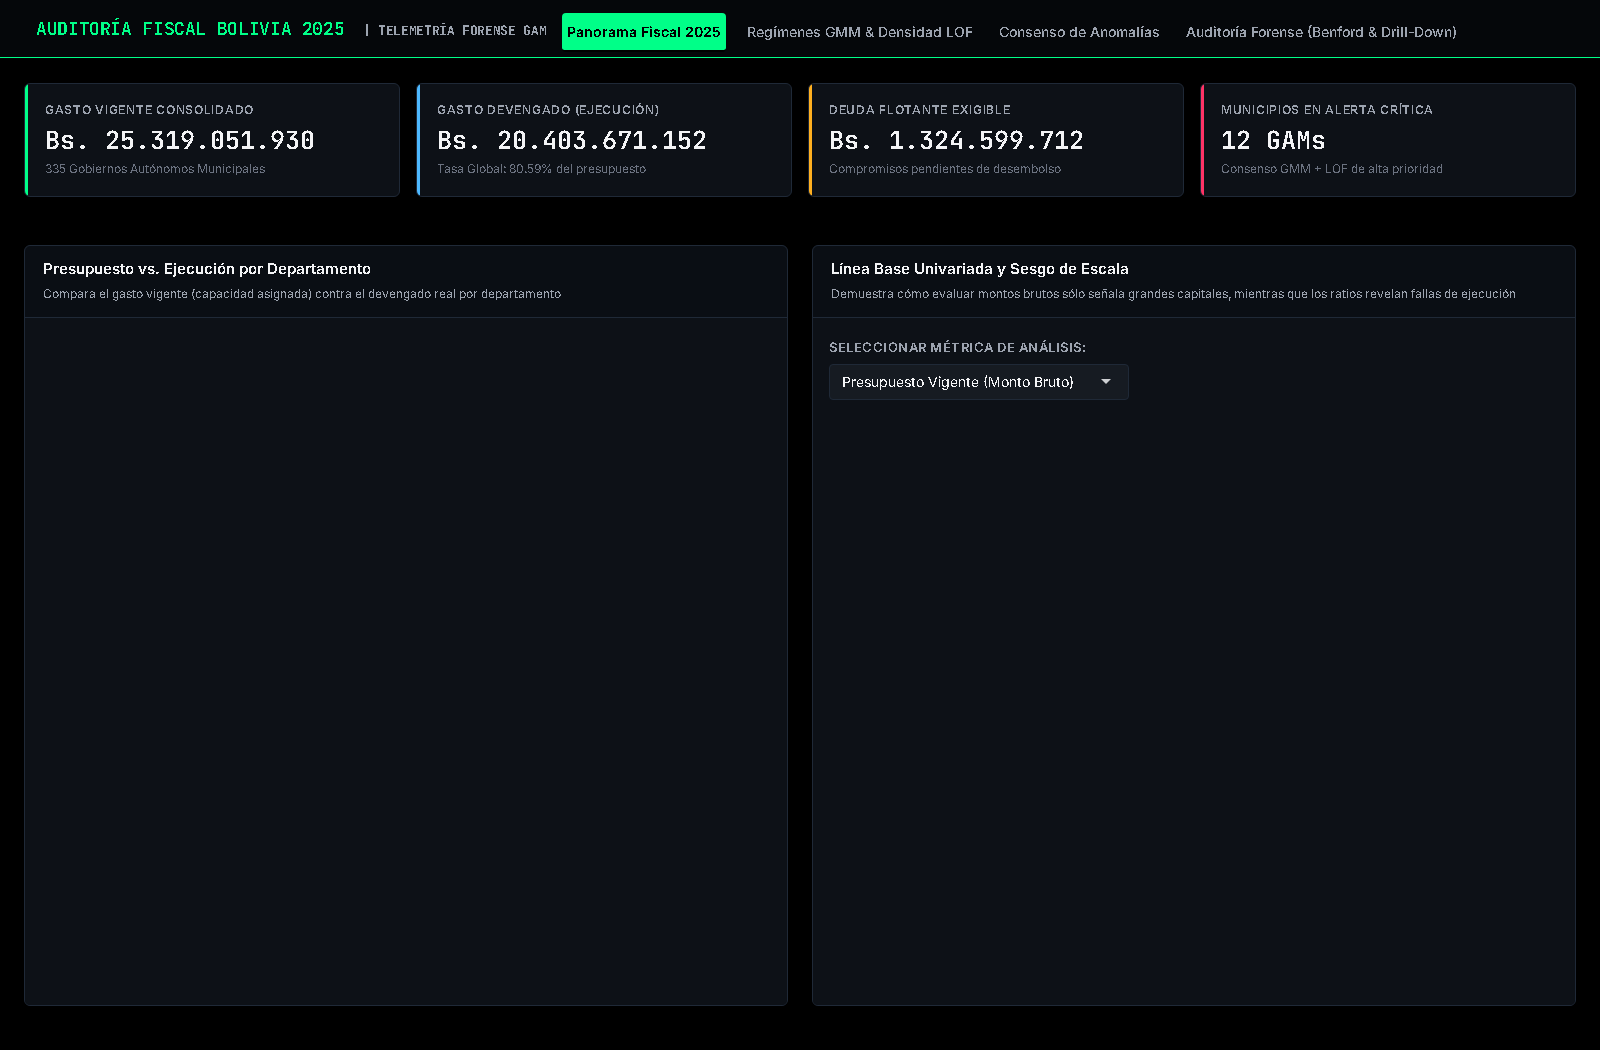
\includegraphics[width=0.92\textwidth]{figuras/dashboard_interactivo_preview.png}
    \caption{Pestaña 1 del Dashboard: Panorama Fiscal 2025, cuadro de mando ejecutivo y módulo interactivo de línea base univariada.}
    \label{fig:dashboard_preview_1}
\end{figure}

\subsubsection{Pestaña 2: Regímenes GMM \& Densidad LOF}
La segunda pestaña (Figura \ref{fig:dashboard_preview_2}) materializa la exploración geométrica de los modelos de aprendizaje no supervisado. En ella se proyecta el espacio latente de Componentes Principales (PCA en 2D y 3D interactivo con WebGL) junto a las elipses de densidad de los 4 regímenes gaussianos estimados por \texttt{mclust}. El auditor dispone de una barra lateral interactiva con controles deslizantes (\textit{sliders}) para modular en tiempo real el tamaño de vecindad $minPts \in [10, 30]$ y el umbral de corte del score LOF (con valor base $1,5$), permitiendo realizar análisis de sensibilidad inmediatos y visualizar qué municipios cambian de estado de atipicidad local.

\begin{figure}[H]
    \centering
    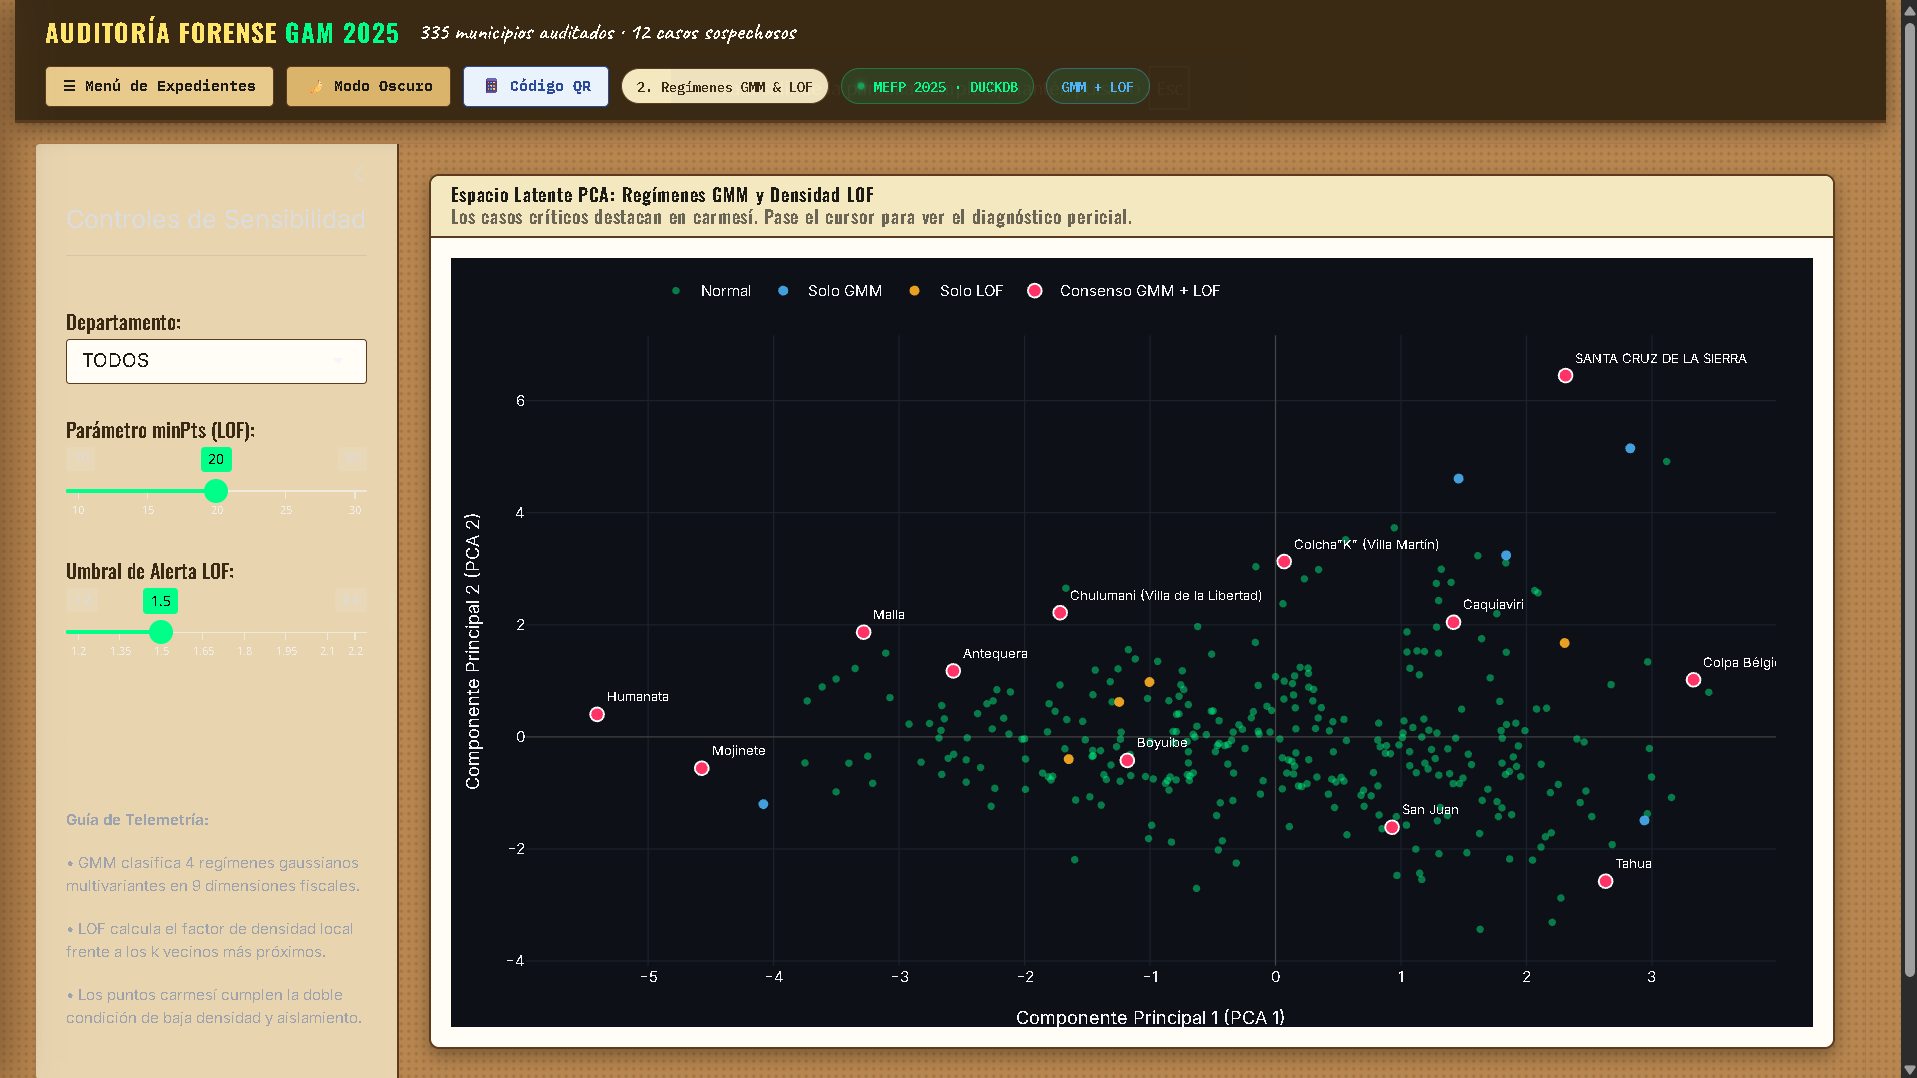
\includegraphics[width=0.92\textwidth]{figuras/dashboard_interactivo_preview_2.png}
    \caption{Pestaña 2 del Dashboard: Regímenes GMM y densidad LOF con proyección multivariante PCA y controles interactivos de sensibilidad.}
    \label{fig:dashboard_preview_2}
\end{figure}

\subsubsection{Pestaña 3: Consenso de Anomalías y Padrón DT}
La tercera pestaña (Figura \ref{fig:dashboard_preview_3}) sintetiza el cruce metodológico de consenso entre el modelo paramétrico GMM y el no paramétrico LOF. Presenta un diagrama de dispersión de cuatro cuadrantes (Log-Densidad GMM vs. Score LOF), destacando en el cuadrante superior izquierdo a los 12 municipios con anomalía simultánea. Debajo se despliega el padrón completo de los 335 GAMs en una tabla interactiva construida con \texttt{DT}, que incluye barras de búsqueda instantánea, paginación, filtros multicriterio por departamento y botones de exportación a formatos abiertos (CSV, Excel, PDF).

\begin{figure}[H]
    \centering
    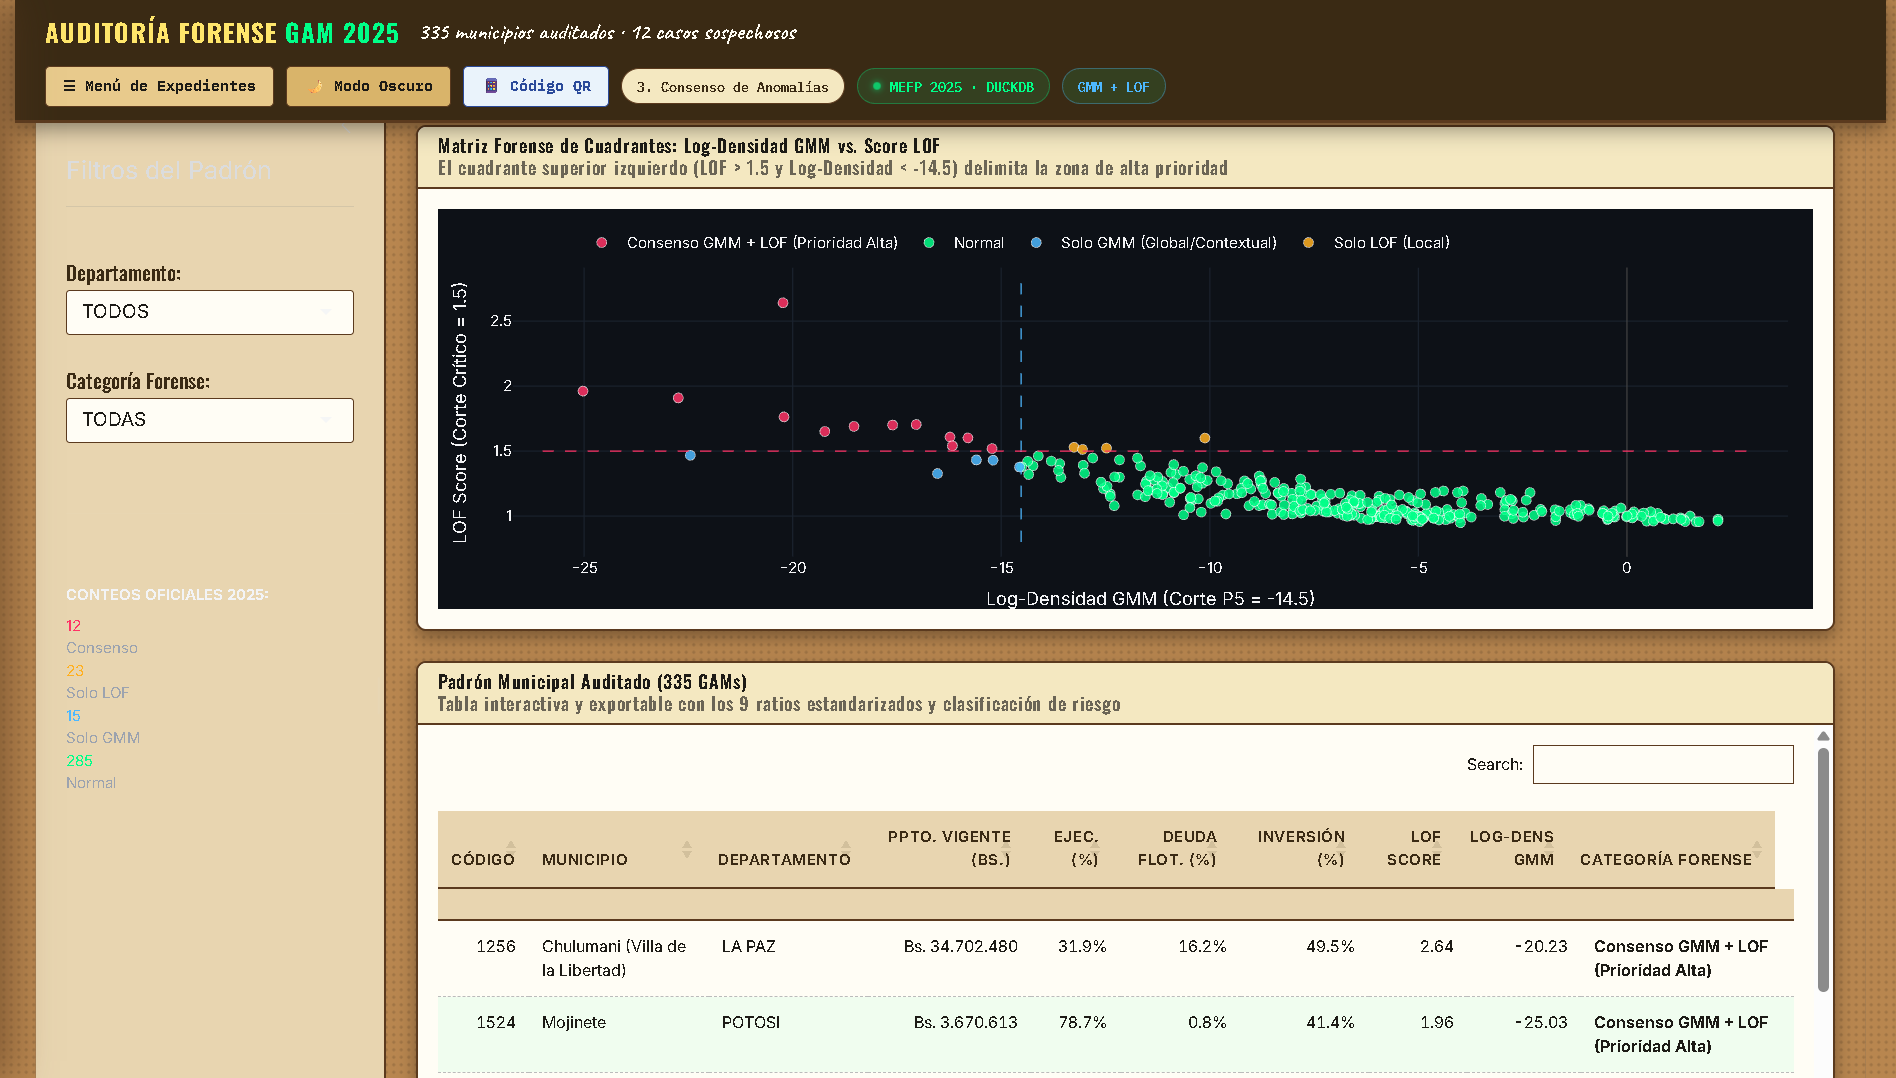
\includegraphics[width=0.92\textwidth]{figuras/dashboard_interactivo_preview_3.png}
    \caption{Pestaña 3 del Dashboard: Matriz de consenso GMM + LOF y tabla analítica interactiva de los 335 GAMs.}
    \label{fig:dashboard_preview_3}
\end{figure}

\subsubsection{Pestaña 4: Expediente de Evidencias Forenses}
La cuarta pestaña (Figura \ref{fig:dashboard_preview_4}) funciona como un módulo de auditoría pericial individual (\textit{drill-down}). Al seleccionar cualquier municipio del país (con accesos directos a los 12 casos de consenso), la plataforma extrae dinámicamente sus comprobantes contables y despliega tres componentes analíticos:
\begin{enumerate}[label=\alph*),noitemsep]
    \item La curva empírica de la Ley de Benford (primer dígito) contrastada con la distribución logarítmica teórica, calculando en tiempo real el estadístico $\chi^2$, el valor $p$ y el MAD de Nigrini.
    \item El gráfico de anillo (\textit{donut chart}) de la composición del gasto devengado por objeto del gasto (Grupos 10000 al 90000).
    \item El balance de liquidez de caja que compara los ingresos percibidos frente a los gastos pagados y la deuda flotante exigible.
\end{enumerate}

\begin{figure}[H]
    \centering
    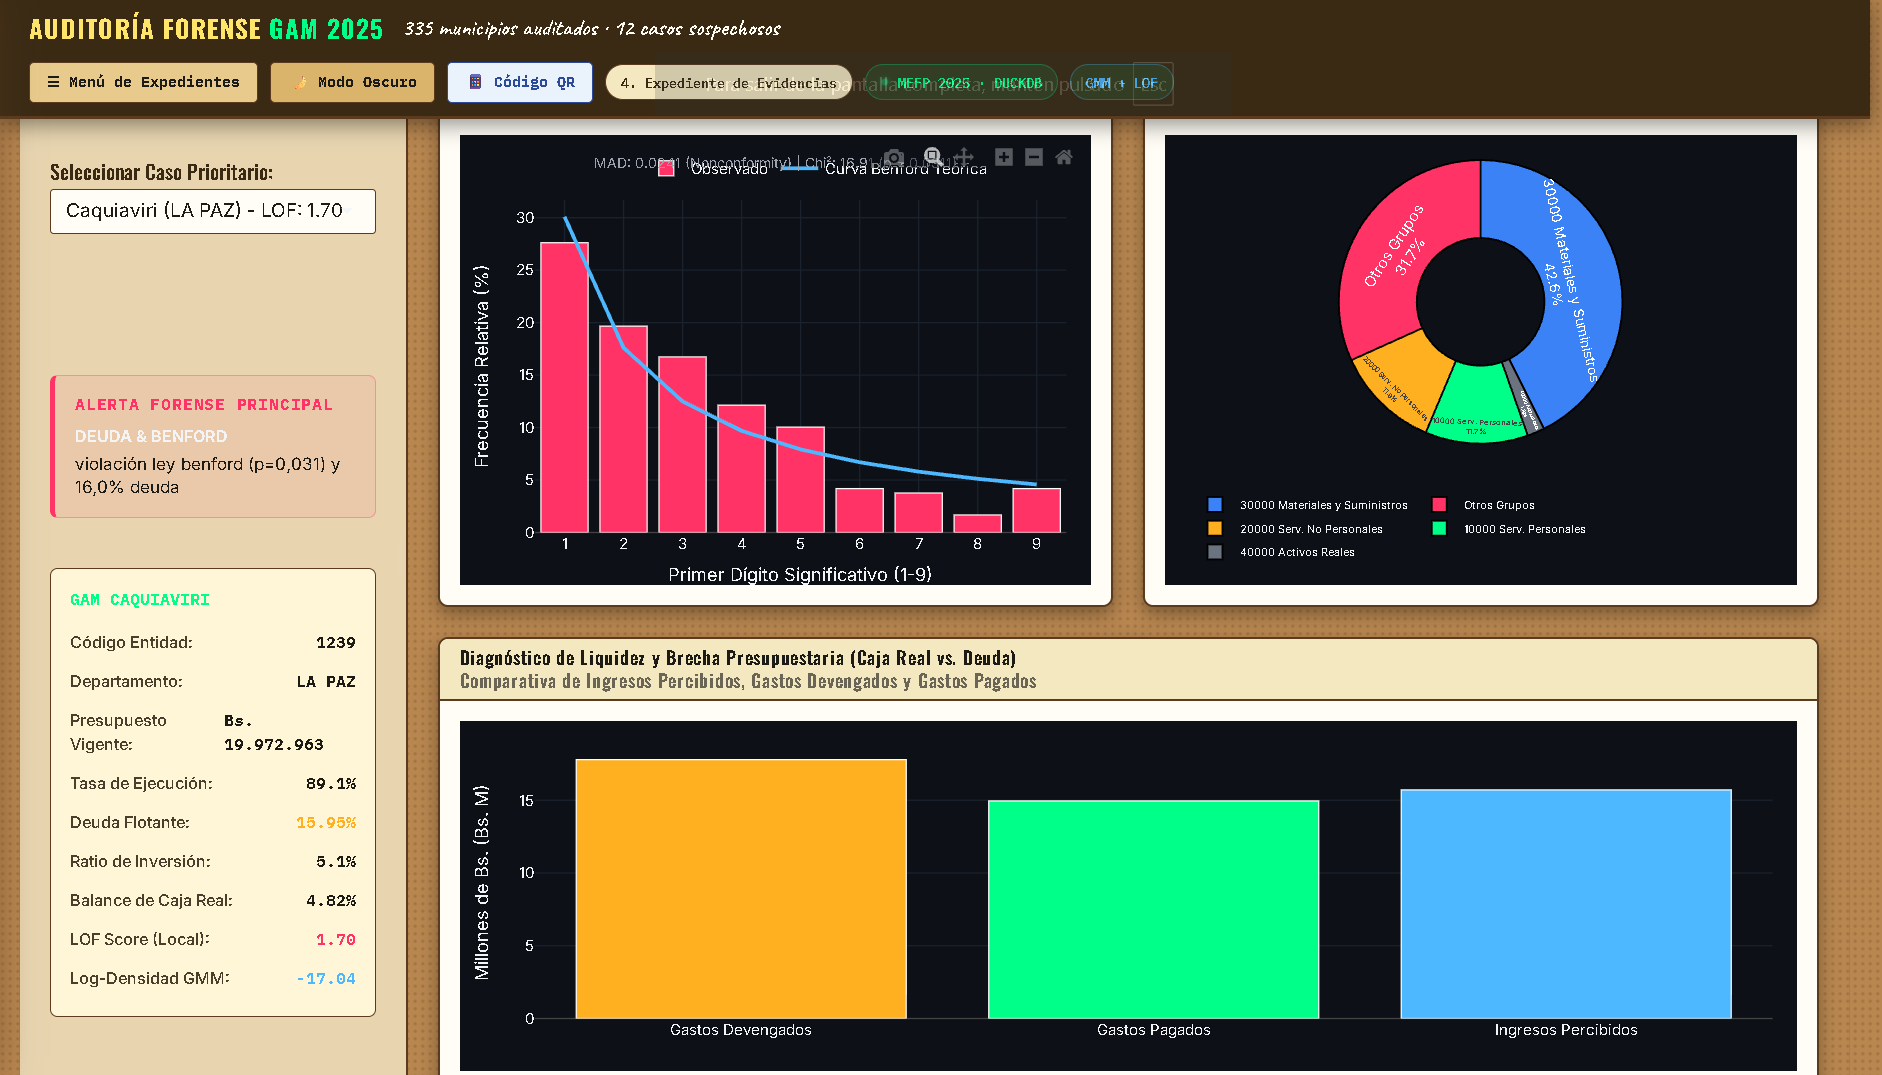
\includegraphics[width=0.92\textwidth]{figuras/dashboard_interactivo_preview_4.png}
    \caption{Pestaña 4 del Dashboard: Expediente forense individual con prueba interactiva de la Ley de Benford y desglose presupuestario.}
    \label{fig:dashboard_preview_4}
\end{figure}

\subsubsection{Pestaña 5: Tablero de Investigación Criminalístico}
La quinta pestaña (Figura \ref{fig:dashboard_preview_5}) implementa la metáfora visual pericial de tablero de corcho desarrollada en los prototipos de \texttt{Ideas/}. Cada uno de los 12 municipios priorizados se representa como una ficha policial/pericial con chinchetas rojas, notas explicativas manuscritas (tipografía \textit{Caveat}), rotaciones orgánicas y su score LOF. Hilos conectores generados en SVG interactivo vinculan automáticamente a los municipios que comparten una misma patología fiscal (deuda e iliquidez, déficit de tesorería, inversión atípica o fraccionamiento de compras), resaltando sus relaciones al pasar el cursor sobre cualquier tarjeta.

\begin{figure}[H]
    \centering
    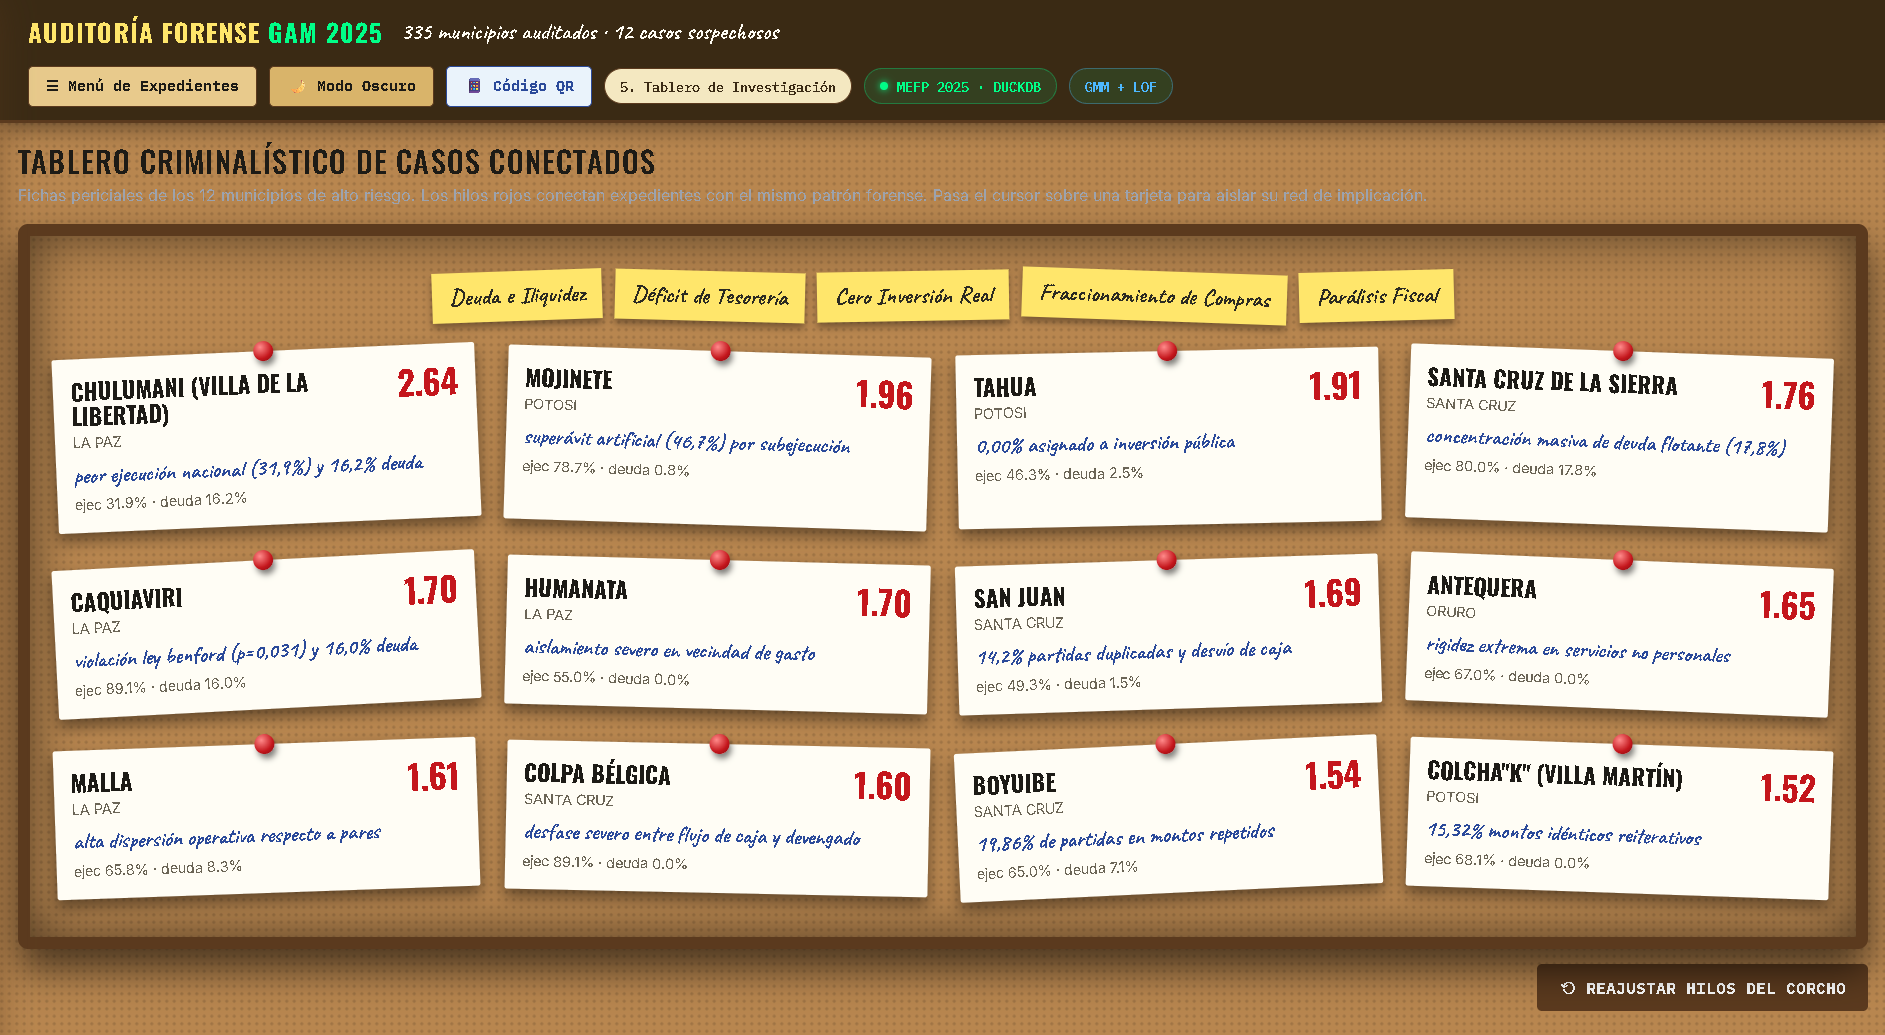
\includegraphics[width=0.92\textwidth]{figuras/dashboard_interactivo_preview_5.png}
    \caption{Pestaña 5 del Dashboard: Tablero de investigación pericial con fichas municipales e hilos conectores por tipología forense.}
    \label{fig:dashboard_preview_5}
\end{figure}

\subsubsection{Pestaña 6: Telemetría Split-Flap y Cinta de Sumadora}
La sexta pestaña (Figura \ref{fig:dashboard_preview_6}) combina dos conceptos visuales de alta densidad técnica: un panel mecánico de llegadas tipo \textit{Split-Flap} (con animación de caracteres alfanuméricos que rotan mecánicamente hasta fijar los valores de los 12 casos atípicos) y un simulador interactivo de cinta de sumadora contable que imprime secuencialmente el resumen fiscal de la auditoría, culminando con el sello pericial de \textit{OBSERVADO}.

\begin{figure}[H]
    \centering
    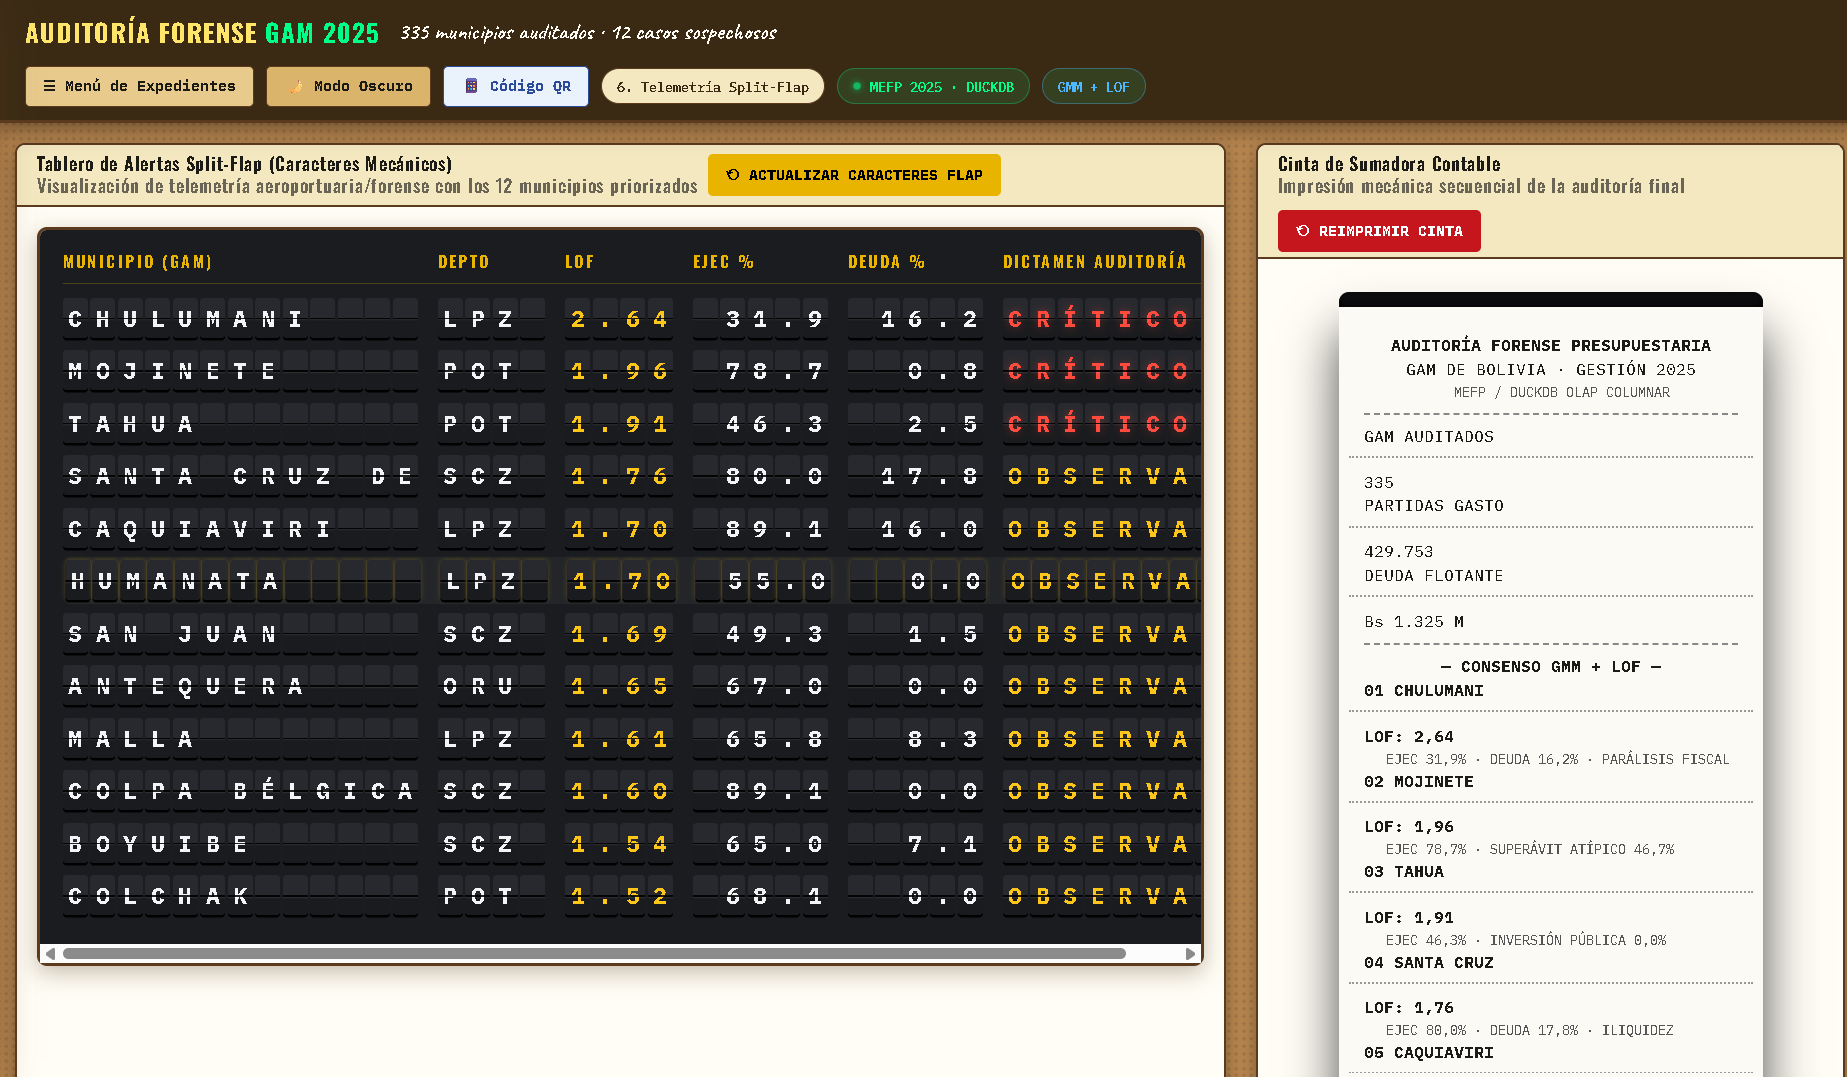
\includegraphics[width=0.92\textwidth]{figuras/dashboard_interactivo_preview_6.png}
    \caption{Pestaña 6 del Dashboard: Módulo de telemetría mecánica Split-Flap y simulación de cinta de sumadora contable.}
    \label{fig:dashboard_preview_6}
\end{figure}

\subsubsection{Pestaña 7: Gráficas Comparativas y Benchmark}
La séptima pestaña (Figura \ref{fig:dashboard_preview_7}) concentra tres análisis comparativos de rendimiento y riesgo:
\begin{enumerate}[label=\alph*),noitemsep]
    \item Gráfico de dispersión bidimensional: Ratio de Inversión Pública vs. Brecha de Pago (Deuda Flotante), con cuadrantes semánticos que diferencian la \textit{Zona de Salud Fiscal} (alta inversión y baja deuda) de la \textit{Zona Crítica} (baja inversión y sobreendeudamiento).
    \item Ranking horizontal del indicador forense MAD de Benford en los 12 municipios en consenso, destacando aquellos que superan el umbral de no conformidad ($0,015$).
    \item Ranking de concentración de montos duplicados reincidentes para identificar alertas de fraccionamiento contractual bajo el D.S. N° 0181.
\end{enumerate}

\begin{figure}[H]
    \centering
    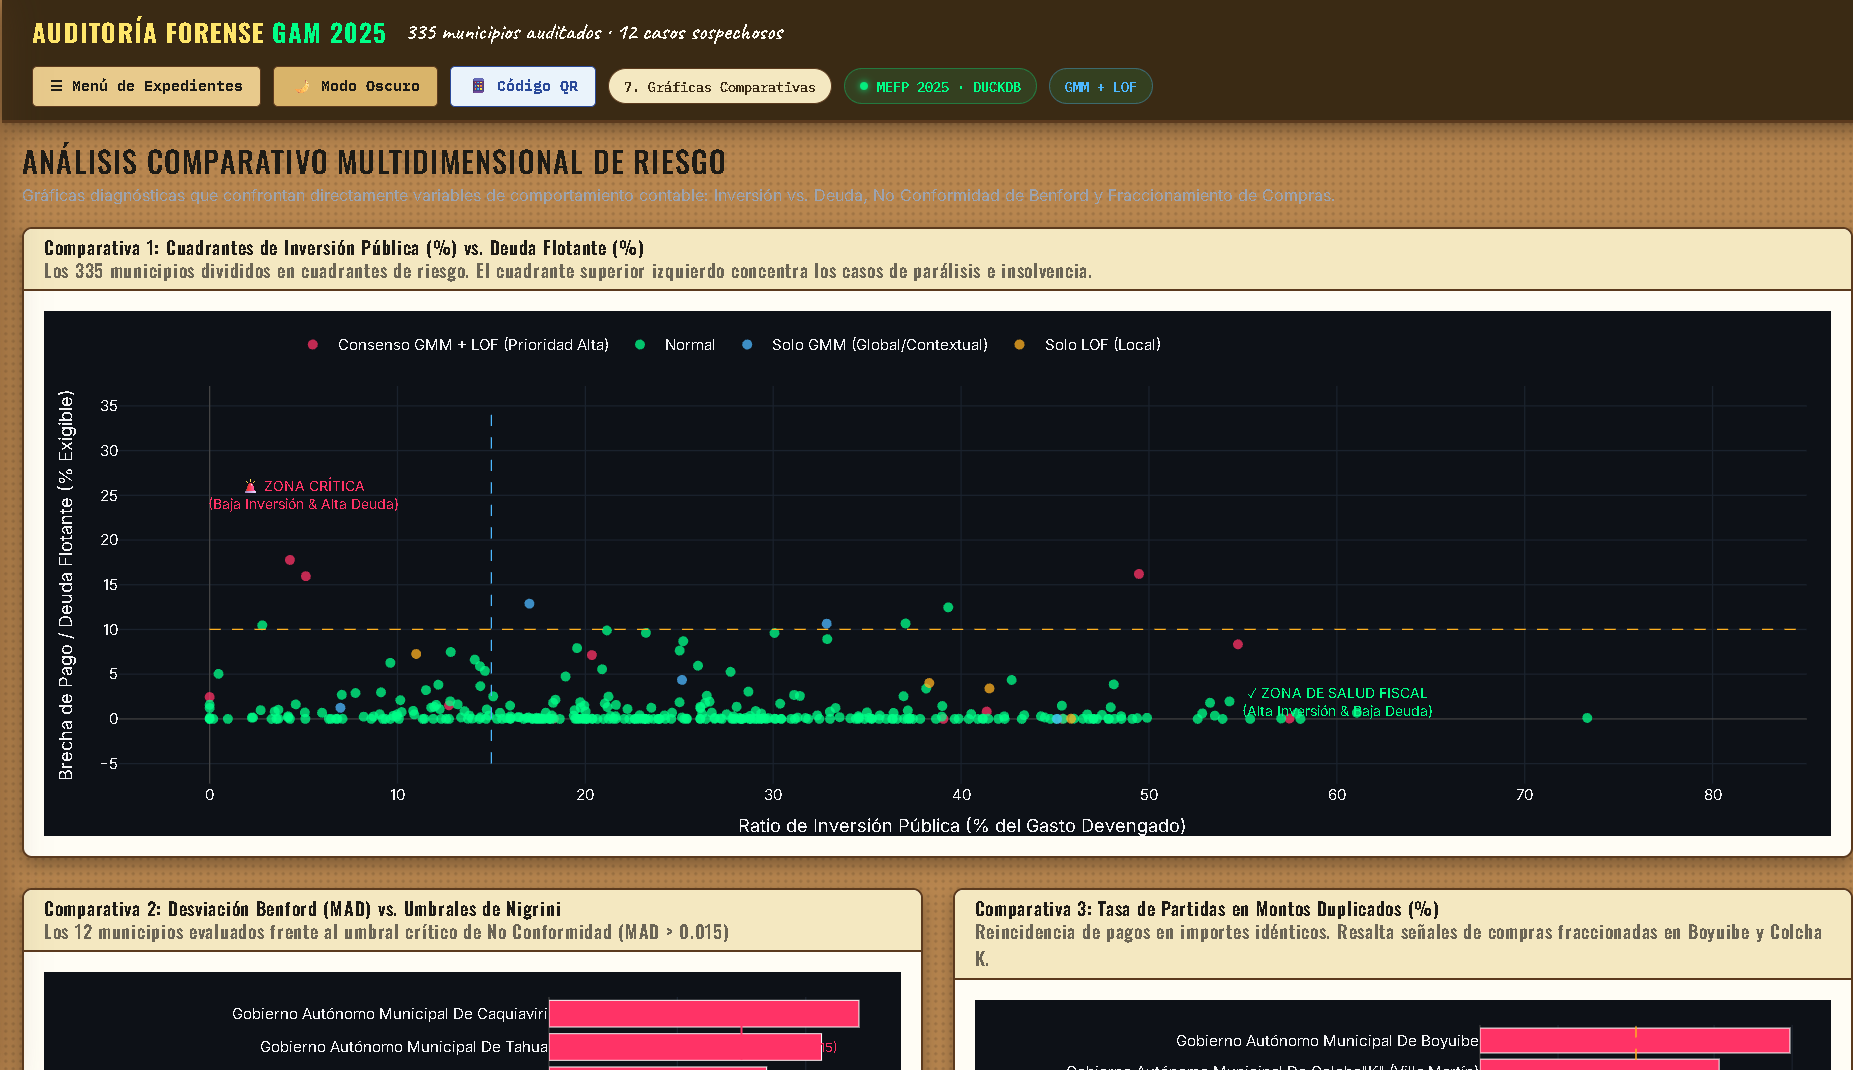
\includegraphics[width=0.92\textwidth]{figuras/dashboard_interactivo_preview_7.png}
    \caption{Pestaña 7 del Dashboard: Gráficas comparativas de cuadrantes de riesgo, ranking MAD de Benford y porcentajes de duplicados.}
    \label{fig:dashboard_preview_7}
\end{figure}

\subsubsection{Pestaña 8: Bitácora KDD \& Evidencias}
La octava pestaña (Figura \ref{fig:dashboard_preview_8}) expone la trazabilidad completa del proceso de Descubrimiento de Conocimiento en Bases de Datos (KDD). Detalla los registros de integridad contable en bruto (reversiones presupuestarias, partidas pagadas por encima de devengados e inconsistencias transaccionales), la documentación formal del clasificador del MEFP y los enlaces directos a las fuentes de datos abiertos y al repositorio de código fuente.

\begin{figure}[H]
    \centering
    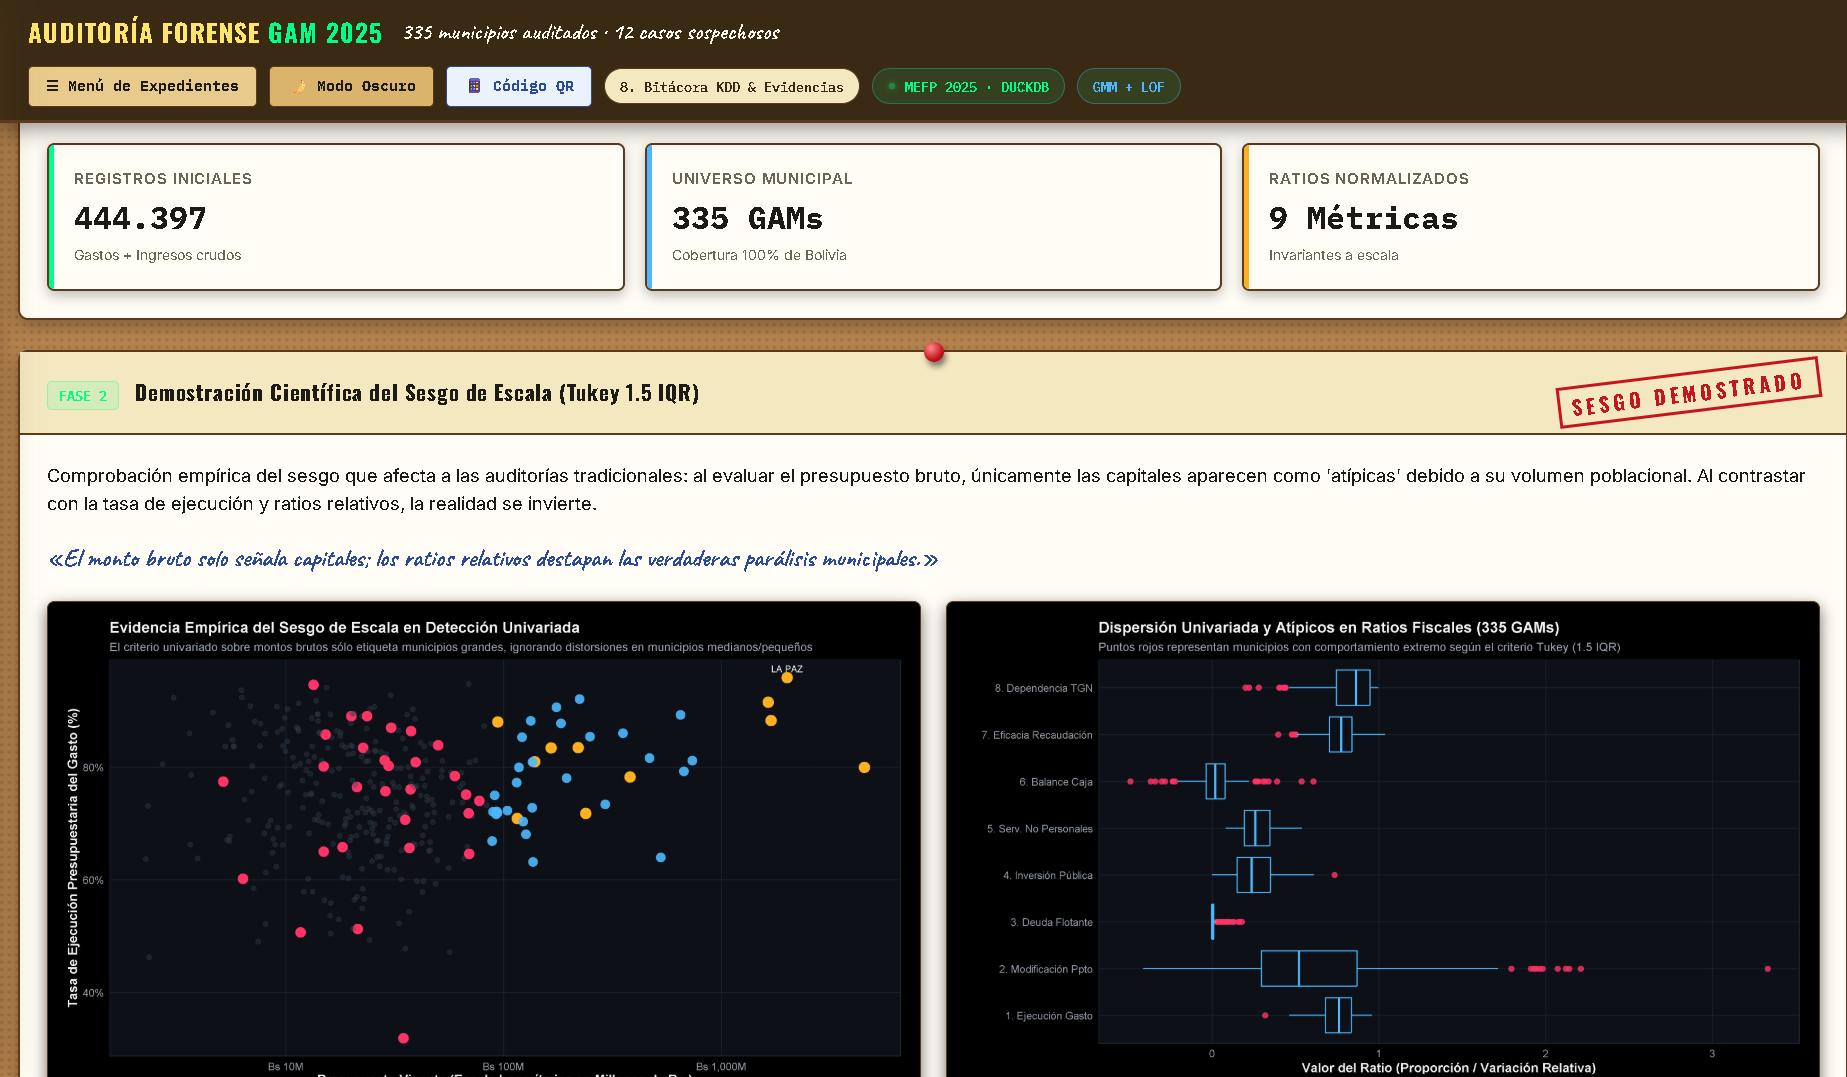
\includegraphics[width=0.92\textwidth]{figuras/dashboard_interactivo_preview_8.png}
    \caption{Pestaña 8 del Dashboard: Bitácora KDD, registro de integridad contable y trazabilidad del proceso analítico.}
    \label{fig:dashboard_preview_8}
\end{figure}

% ------------------------------------------------------------------------------
\section{Conclusiones}
% ------------------------------------------------------------------------------
\begin{enumerate}[label=\textbf{\arabic*.}]
    \item \textbf{Superación del Sesgo de Escala:} Se demostró empíricamente que la fiscalización tradicional sobre montos brutos concentra erróneamente la atención en grandes urbes que operan dentro de parámetros financieros normales, invisibilizando distorsiones operativas y de control en municipios medianos y rurales. La formulación de 9 ratios fiscales relativos permitió una nivelación rigurosa de la escala.
    \item \textbf{Solidez del Consenso Multivariante:} La triangulación de modelos probabilísticos de densidad global (GMM, $G=4$ regímenes) con algoritmos no paramétricos de densidad local (LOF) permitió aislar con precisión estadística a 12 municipios críticos en consenso (3,58\% del universo nacional), cuya condición anómala demostró ser altamente estable frente a variaciones de hiperparámetros ($r > 0,94$).
    \item \textbf{Evidencia Forense Concluyente:} El análisis de microdatos confirmó patologías específicas: Caquiaviri viola la Ley de Benford con significancia estadística ($p=0,031$); Boyuibe, Colcha ``K'' y San Juan concentran entre 14\% y 20\% de sus comprobantes en montos idénticos repetitivos propios de fraccionamiento de compras; Chulumani evidencia parálisis de gestión con recursos estancados; y Tahua asignó 0\% a inversión real en infraestructura.
    \item \textbf{Eficiencia y Transferibilidad Computacional:} El uso de DuckDB en disco procesó más de 444.000 transacciones contables en segundos sin requerir infraestructura computacional de gran escala, y el Dashboard interactivo en Shiny proporciona una herramienta de telemetría directamente transferible a la práctica de la auditoría gubernamental.
\end{enumerate}

% ------------------------------------------------------------------------------
\section{Recomendaciones}
% ------------------------------------------------------------------------------
\begin{enumerate}[label=\textbf{\arabic*.}]
    \item \textbf{A la Contraloría General del Estado (CGE):} Incorporar las rutinas algorítmicas de GMM, LOF y Benford como filtros automatizados de alerta temprana en la planificación anual de auditorías gubernamentales, priorizando inspecciones de campo sobre los municipios que caen en el cuadrante de consenso.
    \item \textbf{Al Ministerio de Economía y Finanzas Públicas (MEFP):} Implementar controles automáticos en el Sistema Integrado de Gestión Pública (SIGEP) que alerten en tiempo real cuando una unidad ejecutora emita comprobantes reiterados en los límites de Contratación Menor (Bs. 20.000 y 50.000) o registre más de un 15\% de deuda flotante acumulada al tercer trimestre.
    \item \textbf{A los Concejos Municipales y Control Social:} Utilizar plataformas interactivas de datos abiertos para supervisar trimestralmente la ejecución de proyectos de inversión real y fiscalizar que los fondos de coparticipación e IDH no se desvíen hacia gastos corrientes en servicios no personales.
    \item \textbf{Líneas Futuras de Investigación:} Extender el modelo multivariante hacia un análisis de series temporales longitudinales (2020--2025) y aplicar técnicas de Procesamiento de Lenguaje Natural (NLP) sobre las glosas descriptivas de los comprobantes contables para detectar redes de proveedores y colusión en licitaciones.
\end{enumerate}

% ------------------------------------------------------------------------------
\section{Bibliografía y Fuentes de Información}
% ------------------------------------------------------------------------------
\bibliographystyle{apalike}
\bibliography{referencias}

\end{document}
